%%!TEX root = dissertation.tex
\setcounter{chapter}{1}
\chapter{The SpiCE Corpus}
\label{ch2:corpus}

\section{Introduction}\label{ch2:sec:introduction}
Much of our formal knowledge about the phonetics of spoken language and speech processing comes from monolingual individuals producing scripted speech in laboratory settings. While far from the only source of knowledge, especially as areas like sociophonetics and corpus phonetics continue to grow, laboratory speech perhaps retains an outsized role. Monolingual lab speech allows researchers to exercise tight control over the linguistic backgrounds of the speakers and the linguistic material (e.g., reading or repeating sounds, words, or sentences). While highly informative, these controlled monolingual speech samples represent a minority of the contexts in which spoken languages are used around the world. Bilingualism is the norm, not the exception, and individuals regularly make creative linguistic choices in their spontaneous speech.\footnote{Throughout this chapter, and in the literature more broadly, multilingualism and bilingualism are used somewhat interchangeably. While there is a growing area focused on trilingualism and language acquisition beyond two languages, multilingualism research tends to focus on two languages.}

Conversational speech allows for a richer empirical description of spoken language compared to---or at the very least, in addition to---laboratory elicited speech. It provides a more realistic representation of how individuals produce language in everyday contexts that isolated word production and sentence reading do not faithfully capture. It enables and facilitates the study of non-formal speech styles, style-shifting, and more. Conversational speech also crucially permits for field testing of speech production theories in their natural habitats. Corpus-based research with conversational or spontaneous speech is important in the fields of phonetics and psycholinguistics, as the research conclusions drawn from corpus and lab-based experiments do not always coincide, given the differences in communicative contexts, attentional demands, and speaking rate variability \citep[e.g.,][]{gahl_2012_reduce,johnson_2021_language}. 

Discrepancies between results for conversational and lab speech have been found for monolingual (English) speech but are likely to be found with bilingual speech as well. Research on bilingual conversational speech is limited, however, as the resources needed for this type of inquiry are relatively rare. Furthermore, the corpora that do exist have typically focused on bilinguals of two European languages.

As a step towards filling this gap, this chapter introduces the \textbf{SpiCE} corpus of conversational bilingual \textbf{Sp}eech \textbf{i}n \textbf{C}antonese and \textbf{E}nglish \citep{johnson_2021_spice}. In contributing to filling this gap, SpiCE will allow researchers to address a set of research questions that were previously not possible, using both conversational, bilingual speech, and sophisticated phonetic measurements at scale. To preview the end product before diving into the details---SpiCE is a corpus of bilingual speech in Cantonese and English, comprising high-quality recordings of 34 early Cantonese-English bilinguals. The participants were young adult members of the heterogeneous bilingual speech community in the Vancouver, BC, Canada, area. Each participant completed a few different tasks—reading sentences, narrating a cartoon storyboard, and conversing freely in a semi-structured interview with a bilingual peer as the interviewer. All of the recordings were manually transcribed at the word level and force-aligned at the phone level. This chapter describes each of these components in detail and offers justification for the decisions where warranted.

The SpiCE corpus design is based on key aspects of widely used existing spontaneous speech corpora, such as the Buckeye corpus of conversational speech \citep{pitt_2005_buckeye}. In many ways, the Buckeye corpus is treated as a gold standard in the field of corpus phonetics. And while the SpiCE corpus does not copy its structure and level of detail exactly, the Buckeye corpus nonetheless serves as inspiration, particularly given its casual interview style and high recording quality. The goal, after all, is to facilitate phonetics research with spontaneous bilingual speech. 

Given the bilingual design, SpiCE crucially includes speech from the same individual in more than one language. Inspiration in this regard is drawn from the Bangor corpora of Spanish-English, Welsh-English, and Welsh-Spanish bilingual speech \citep{deuchar_2014_corpora}. The Bangor corpora include speech from the same individual in more than one language but largely comprise field recordings, some of which are noisy. For example, many of the recordings in the Spanish-English Bangor corpus were made with a lapel microphone worn on the participant's belt and others with a radio microphone placed on a table. This variable---and often noisy---recording quality limits the scope of phonetics research using the corpora. Additionally, the Bangor corpora were designed for understanding code-switching in everyday situations. While this facilitates understanding broad patterns of language use, it also means that the corpora are not necessarily balanced for the languages involved---people do not necessarily use their languages in equal proportions. So while these corpora are incredibly valuable for linguistics research, there are nonetheless limitations. Compared to these corpora, SpiCE uses a more controlled and balanced recording setup, which allows for more nuanced acoustic-phonetic measurements. This is, however, at the expense of other criteria (e.g., naturalness), in which the Bangor corpora excel.

The SpiCE corpus was initially designed in mid-2018, with recording beginning in the fall of 2018. At that time, there were relatively few corpora comprising multilingual speech. There has been a notable uptick in the development of such corpora since that time. For example, there was a session at the 2018 Langauge Resources and Evaluation Conference on ``Bilingual Speech Corpora and Code-switching.''\footnote{\url{http://www.lrec-conf.org/proceedings/lrec2018/sessions.html}} In a similar vein, Microsoft hosted the ``First Workshop on Speech Technologies for Code-switching in Multilingual Communities'' in conjunction with Interspeech 2020.\footnote{\url{https://www.microsoft.com/en-us/research/event/workshop-on-speech-technologies-for-code-switching-2020/}} These workshops are examples of the growing interest in working with multilingual speech data at larger scales. It parallels the similarly large growth of corpus phonetics as a field \citep{liberman_2019_corpus,grieve_2021_observation}.

SpiCE is also unique in the population it represents. Many of the resources available to researchers on sites like BilingBank, ELRA, and elsewhere feature late bilinguals and second language learners and vary widely in task and recording quality. One example of a Cantonese-English resource that fits this description is the ShefCE corpus \citep{ng_shefce_2017}. ShefCE is a parallel corpus featuring L1 Hong Kong Cantonese and L2 English read speech, where participants read lectures in each language one sentence at a time. While there are similarities with what SpiCE aims to accomplish (e.g., promoting research with Cantonese-English bilingual speech), ShefCE occupies a different niche in the speech sciences---it was designed for L2 pronunciation assessment and training speech recognition models. Another resource focused on bilinguals L1 Cantonese and L2 English is the ALLSSTAR corpus---Archive of L1 and L2 Scripted and Spontaneous Transcripts And Recordings---of which Cantonese L1 talkers represent 14 of 140 people for whom English is their L2 \citep{bradlow_2011_allsstar}. 

The primary motivation for collecting this corpus was to have comparable high-quality recordings of conversational speech from early bilinguals in two languages, which enables large-scale phonetic analysis on a within-speaker basis. It is worth noting that corpus size is a subjective measure, as different fields have different standards in this respect. For the type of corpus, SpiCE is relatively large (32.8 total recording hours and approximately 219,000 words), being slightly smaller in size than the Buckeye corpus \citep[approximately 40 total recording hours and 307,000 words][]{pitt_2005_buckeye}. Both of these are purpose-built corpora recorded in person. Truly large corpora tend to be collected from existing recordings \citep[radio, YouTube, audiobooks, etc.; e.g., Librispeech, 1000 hours:][]{panayotov_librispeech_2015}, crowdsourced online \citep[e.g. Mozilla Common Voice, 2500 hours:][]{ardila_2020_common}, via phone \citep[e.g., SWITCHBOARD, 260 hours:][]{godfrey_switchboard_1992}, and other similar more scalable methods. The reason? High-quality, purpose-built corpora are expensive and time-consuming to create.

To my knowledge, this type of resource does not yet exist for any pair of languages, much less for a typologically distinct pair like Cantonese (Sino-Tibetan) and English (Indo-European). Furthermore, Cantonese is a relatively understudied language, despite there being approximately 85 million speakers around the world \citep{ethnologue_yue_2021}, though this is changing with new Cantonese language corpora \citep{luke_2015_hkc, leung_2001_hkcac, winterstein_2020_cantomap, alderete_2019_tone}, natural language processing tools \citep{lee_2018_pycantonese,yau_2019_pyjyutping}, and support in speech technology applications \citep{google_2019_stt}.

While some of the design choices have been touched upon already, the remainder of this chapter provides a detailed overview of the corpus. Sections \ref{ch2:sec:design} covers the design and collection procedures and includes a detailed description of the participants. Section \ref{ch2:sec:annotation} describes the transcription and annotation pipeline. Section \ref{ch2:sec:statistics} concludes with descriptive statistics summarizing the corpus. 

\section{Corpus design and creation}\label{ch2:sec:design}

This section provides detail about the speakers (Section \ref{ch2:subsec:participants}), the procedures used to ensure high-quality recordings (Section \ref{ch2:subsec:setup}), and the three tasks that each participant completed in both Cantonese and English (Section \ref{ch2:subsec:procedure}). 

Data collection took place between November 2018 and March 2020. Orthographic transcription began shortly after the first interview was recorded and was completed in April 2021. The corpus was made available to the public in May 2021 via Scholars Portal Dataverse at \url{https://doi.org/10.5683/SP2/MJOXP3}. Additionally, detailed documentation for the corpus is available both with the corpus download and at \url{https://spice-corpus.readthedocs.io/}.

\subsection{Recruitment}

Participants were recruited for the SpiCE corpus through a variety of methods at the University of British Columbia. This included word of mouth, the Linguistics Human Subject Pool, the Psychology Paid Studies list, advertisements in department email lists, advertisements in linguistics courses, printed flyers, and posts on various club forums. 

The recruitment process focused on fluent speakers of Cantonese and English, between the ages of 19 and 35, with normal speech and hearing, who began learning both languages from early childhood (age five or earlier). One goal of recruitment was to maintain a balance of male- and female-identifying speakers, and as a result, once 17 females had participated, the recruitment language was adjusted to focus on male- or nonbinary-identifying participants.

Before scheduling a session, participants first completed a language background survey. If an individual signed up to participate but did not meet the criteria for participation, their session was canceled, and they were contacted with an explanation.

All participants who came into the lab were compensated for their time with partial course credit or \$15 CAD. 

\subsection{Participants}\label{ch2:subsec:participants} 
The recordings in SpiCE comprise the speech of 34 early Cantonese-English bilinguals. Throughout this chapter and the corpus, participants are identified by participant IDs. The IDs are designed to provide basic information about the participant. For example, VF19A indicates that the participant was recorded in \textbf{V}ancouver, identified as \textbf{F}emale, and was 19 years old at the time of recording. The letter at the end distinguishes participants of the same age and gender. There were 17 participants who self-identified as female and 17 as male. Participants ranged in age from 19 to 34 years old at the time of recording. Apart from one talker who reported mild high-frequency hearing loss (VM25A), all participants reported normal speech and hearing. Additionally, all participants resided in the Metro Vancouver, BC, Canada, area at the time of recording. The SpiCE corpus also includes a detailed summary extracted from an extensive language background survey administered before the recording session (without the researchers present), as well as a copy of the survey itself. Basic summary information is included in Table \ref{ch2:tab:participants}, and in visualizations throughout this chapter. All participant information is based on self-reported participant data from the survey.

There were a handful of additional individuals who participated in the study but were ultimately excluded from the published SpiCE corpus due to missing language background questionnaire information (n=1), recording issues (n=2), or not starting learning Cantonese until age eight (n=1).

\begin{table}[!htbp]
  \begin{center}
    \footnotesize
      \begin{tabular}{ccccccc}
  \toprule
    & & & &                & \multicolumn{2}{c}{\textbf{Age of Acquisition}} \\
  \textbf{No.} & \textbf{ID} & \textbf{Order} & \textbf{Age} & \textbf{Gender} & \textbf{English} & \textbf{Cantonese} \\
  \midrule
  1 & VF19A & E $\rightarrow$ C & 19  & F & 0   & 0 \\
  2 & VF19B & E $\rightarrow$ C & 19  & F & 0   & 0 \\
  3 & VF19C & E $\rightarrow$ C & 19  & F & 3   & 0 \\
  4 & VF19D & C $\rightarrow$ E & 19  & F & 2   & 0 \\
  5 & VF20A & C $\rightarrow$ E & 20  & F & 4   & 0 \\
  6 & VF20B & C $\rightarrow$ E & 20  & F & 5   & 0 \\
  7 & VF21A & E $\rightarrow$ C & 21  & F & 0   & 0 \\
  8 & VF21B & C $\rightarrow$ E & 21  & F & 3   & 0 \\
  9 & VF21C & C $\rightarrow$ E & 21  & F & 4   & 0 \\
  10  & VF21D & E $\rightarrow$ C & 21  & F & 0   & 0 \\
  11  & VF22A & C $\rightarrow$ E & 22  & F & 0   & 0 \\
  12  & VF23B & E $\rightarrow$ C & 23  & F & 2   & 0 \\
  13  & VF23C & C $\rightarrow$ E & 23  & F & 0   & 0 \\
  14  & VF26A & C $\rightarrow$ E & 26  & F & 0   & 0 \\
  15  & VF27A & E $\rightarrow$ C & 27  & F & 0   & 0 \\
  16  & VF32A & C $\rightarrow$ E & 32  & F & 3   & 0 \\
  17  & VF33B & C $\rightarrow$ E & 33  & F & 0   & 0 \\
  18  & VM19A & E $\rightarrow$ C & 19  & M & 0   & 0 \\
  19  & VM19B & C $\rightarrow$ E & 19  & M & 2   & 0 \\
  20  & VM19C & E $\rightarrow$ C & 19  & M & 0   & 0 \\
  21  & VM19D & C $\rightarrow$ E & 18  & M & 1   & 1 \\
  22  & VM20B & E $\rightarrow$ C & 20  & M & 0   & 0 \\
  23  & VM21A & E $\rightarrow$ C & 21  & M & 0   & 0 \\
  24  & VM21B & E $\rightarrow$ C & 21  & M & 0   & 0 \\
  25  & VM21C & C $\rightarrow$ E & 21  & M & 0   & 0 \\
  26  & VM21D & C $\rightarrow$ E & 21  & M & 0   & 0 \\
  27  & VM21E & C $\rightarrow$ E & 21  & M & 5   & 0 \\
  28  & VM22A & C $\rightarrow$ E & 22  & M & 4   & 0 \\
  29  & VM22B & E $\rightarrow$ C & 22  & M & 0   & 0 \\
  30  & VM23A & E $\rightarrow$ C & 23  & M & 0   & 0 \\
  31  & VM24A & E $\rightarrow$ C & 24  & M & 3   & 0 \\
  32  & VM25A & E $\rightarrow$ C & 25  & M & 4   & 0 \\
  33  & VM25B & E $\rightarrow$ C & 25  & M & 0   & 0 \\
  34  & VM34A & C $\rightarrow$ E & 34  & M & 0   & 0 \\
  \bottomrule
  
  \end{tabular}
  \caption{Basic participant information from the language background survey, including age, gender (M for male and F for female), age of acquisition (phrased as ``age began learning''), and the order the interviews occurred (E for English and C for Cantonese). See Section \ref{ch2:subsec:procedure} for information about interview order.}
  \label{ch2:tab:participants}
  \end{center}
  \end{table}

Definitions of bilingualism are highly variable in the literature, as there are many different types of bilinguals \citep{amengual_2017_type}. For this corpus, an early bilingual is someone who began learning both Cantonese and English before starting primary school (approximately age 5), reports consistent use of both languages since that time, and self-selected to participate in a research study involving an interview in each language. It is important to highlight that the Cantonese-English bilingual community in Vancouver (and Canada more generally) is incredibly diverse, both in terms of dialects or varieties spoken, as well as in the regions from which families originally emigrated \citep{yu_2013_diaspora}. Furthermore, given the prevalence of Cantonese in Vancouver \citep{statistics_2017_proportion} and longevity of the community's presence in Vancouver \citep{yu_2013_diaspora}, immigration from other Cantonese-speaking areas continues today. 

This corpus reflects the diverse nature of Cantonese-English bilingualism in Vancouver, as it includes Canadian-born heritage speakers, recent immigrants from Hong Kong, Cantonese speakers from other parts of the Cantonese diaspora, and individuals who do not neatly fit into these particular categories. As a result, while all speakers are early bilinguals, various dialects are represented. Figure \ref{ch2:fig:placeslived} depicts where SpiCE participants reported living during different age intervals. These intervals were selected after reviewing freeform participant responses comprising when they lived in different places. Specifically, Figure \ref{ch2:fig:placeslived} reports the number of participants who indicated that they lived in a given country during the age ranged for the panel. For example, if a participant moved from Hong Kong to Canada at age 7, they would be counted in both bars in that panel. 

\begin{figure}[!htbp]
  \begin{center}
  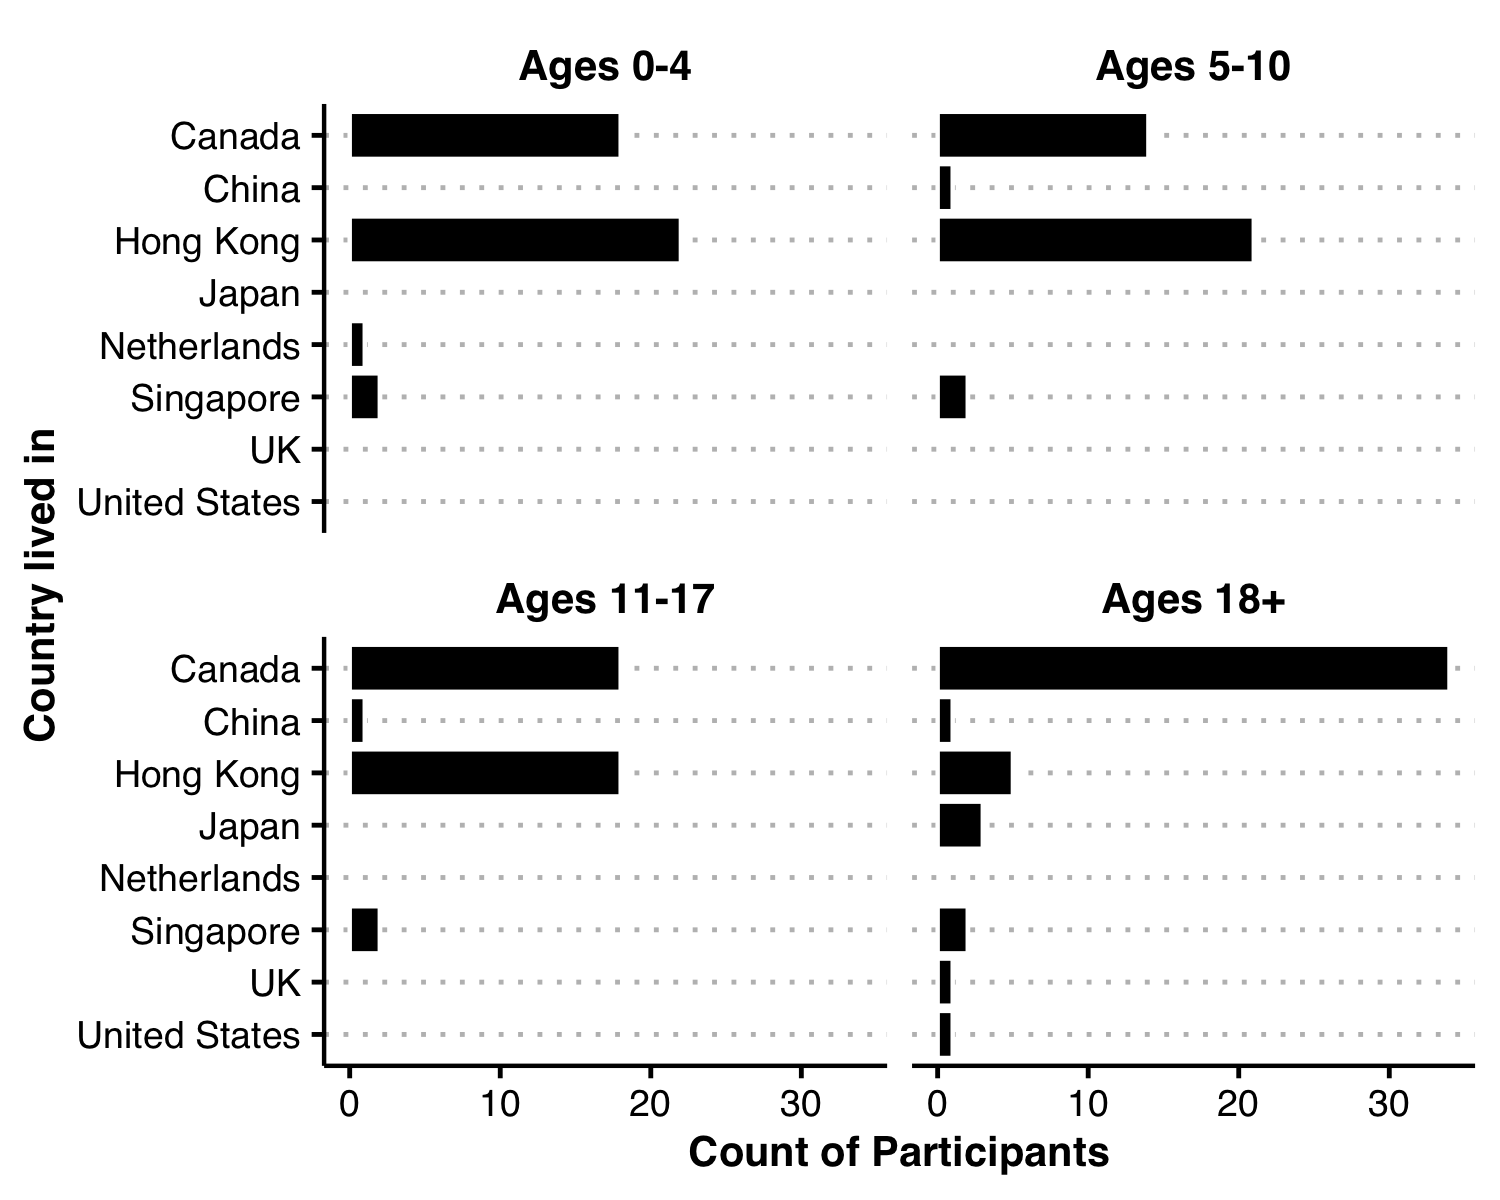
\includegraphics[width=4.9in]{figures/ch2_placeslived_5in.png} 
  \caption{This four panel bar chart summarizes where the SpiCE participants lived during different portions of their lives.}
  \label{ch2:fig:placeslived}
  \end{center}
\end{figure}

Directly soliciting Cantonese dialect information would have been challenging, as many of the participants in the corpus would not have straightforward dialect classifications. This is especially true for individuals who were born and/or raised in the Cantonese diaspora, but to Hong Kongers as well, given the extent of multilingualism and globalization in Hong Kong \citep{bolton_2020_societal}. In light of this, it is useful to summarize where the SpiCE participants' caretakers were primarily raised. Figure \ref{ch2:fig:caretakers} does exactly this. The most well-represented group is Hong Kong, as 29 of 34 participants reported having at least one caretaker who was primarily raised in Hong Kong. Of these, 20 report only having caretakers raised in Hong Kong. If caretaker birth location is considered instead, the numbers are 27 and 18, respectively. 

\begin{figure}[!htbp]
  \begin{center}
  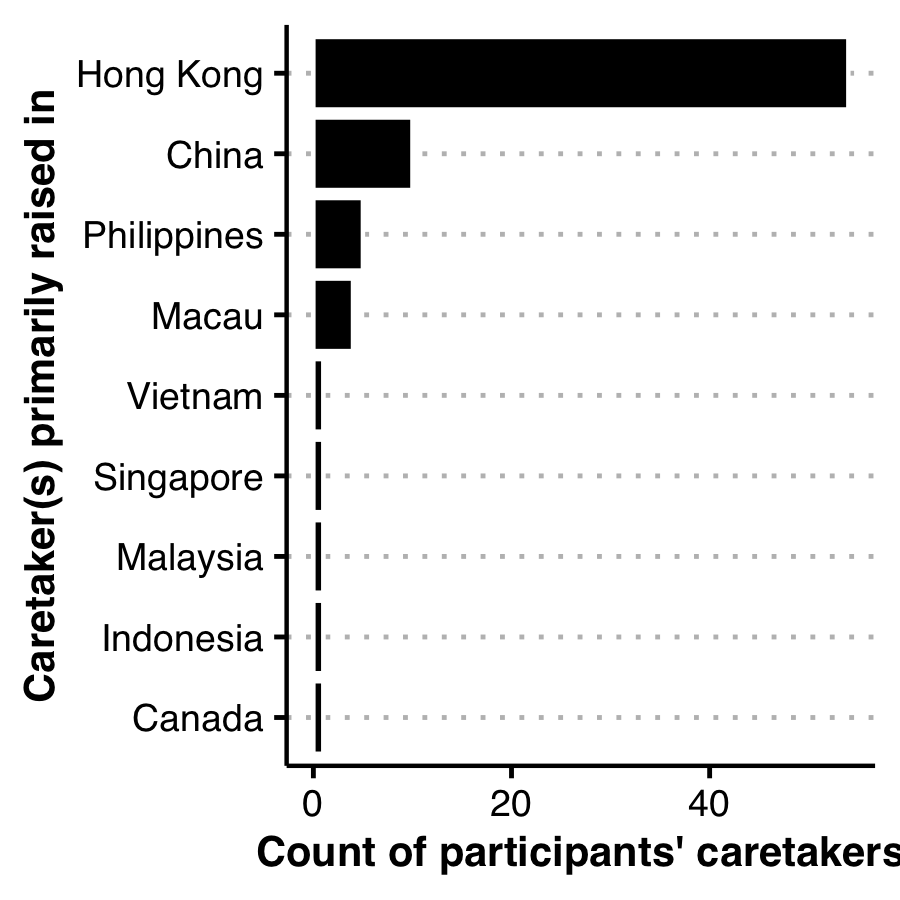
\includegraphics[width=3in]{figures/ch2_caretakers_3in.png} 
  \caption{This bar chart summarizes the number of caretakers who were raised in various locations. Note that the number of caretakers reported by individual participants varies.}
  \label{ch2:fig:caretakers}
  \end{center}
\end{figure}

Additionally, calling an individual a bilingual does not preclude knowledge of additional languages. All but one of the individuals represented in the SpiCE corpus report some degree of proficiency in a language other than Cantonese or English. The most common by far is Mandarin. The age SpiCE talkers began learning other languages varies widely but is consistently later than (or simultaneous with) Cantonese and English. This information is depicted in Figures \ref{ch2:fig:multilingualism_vf} and \ref{ch2:fig:multilingualism_vm}, with a panel for each participant.

\begin{figure}[!htbp]
  \begin{center}
  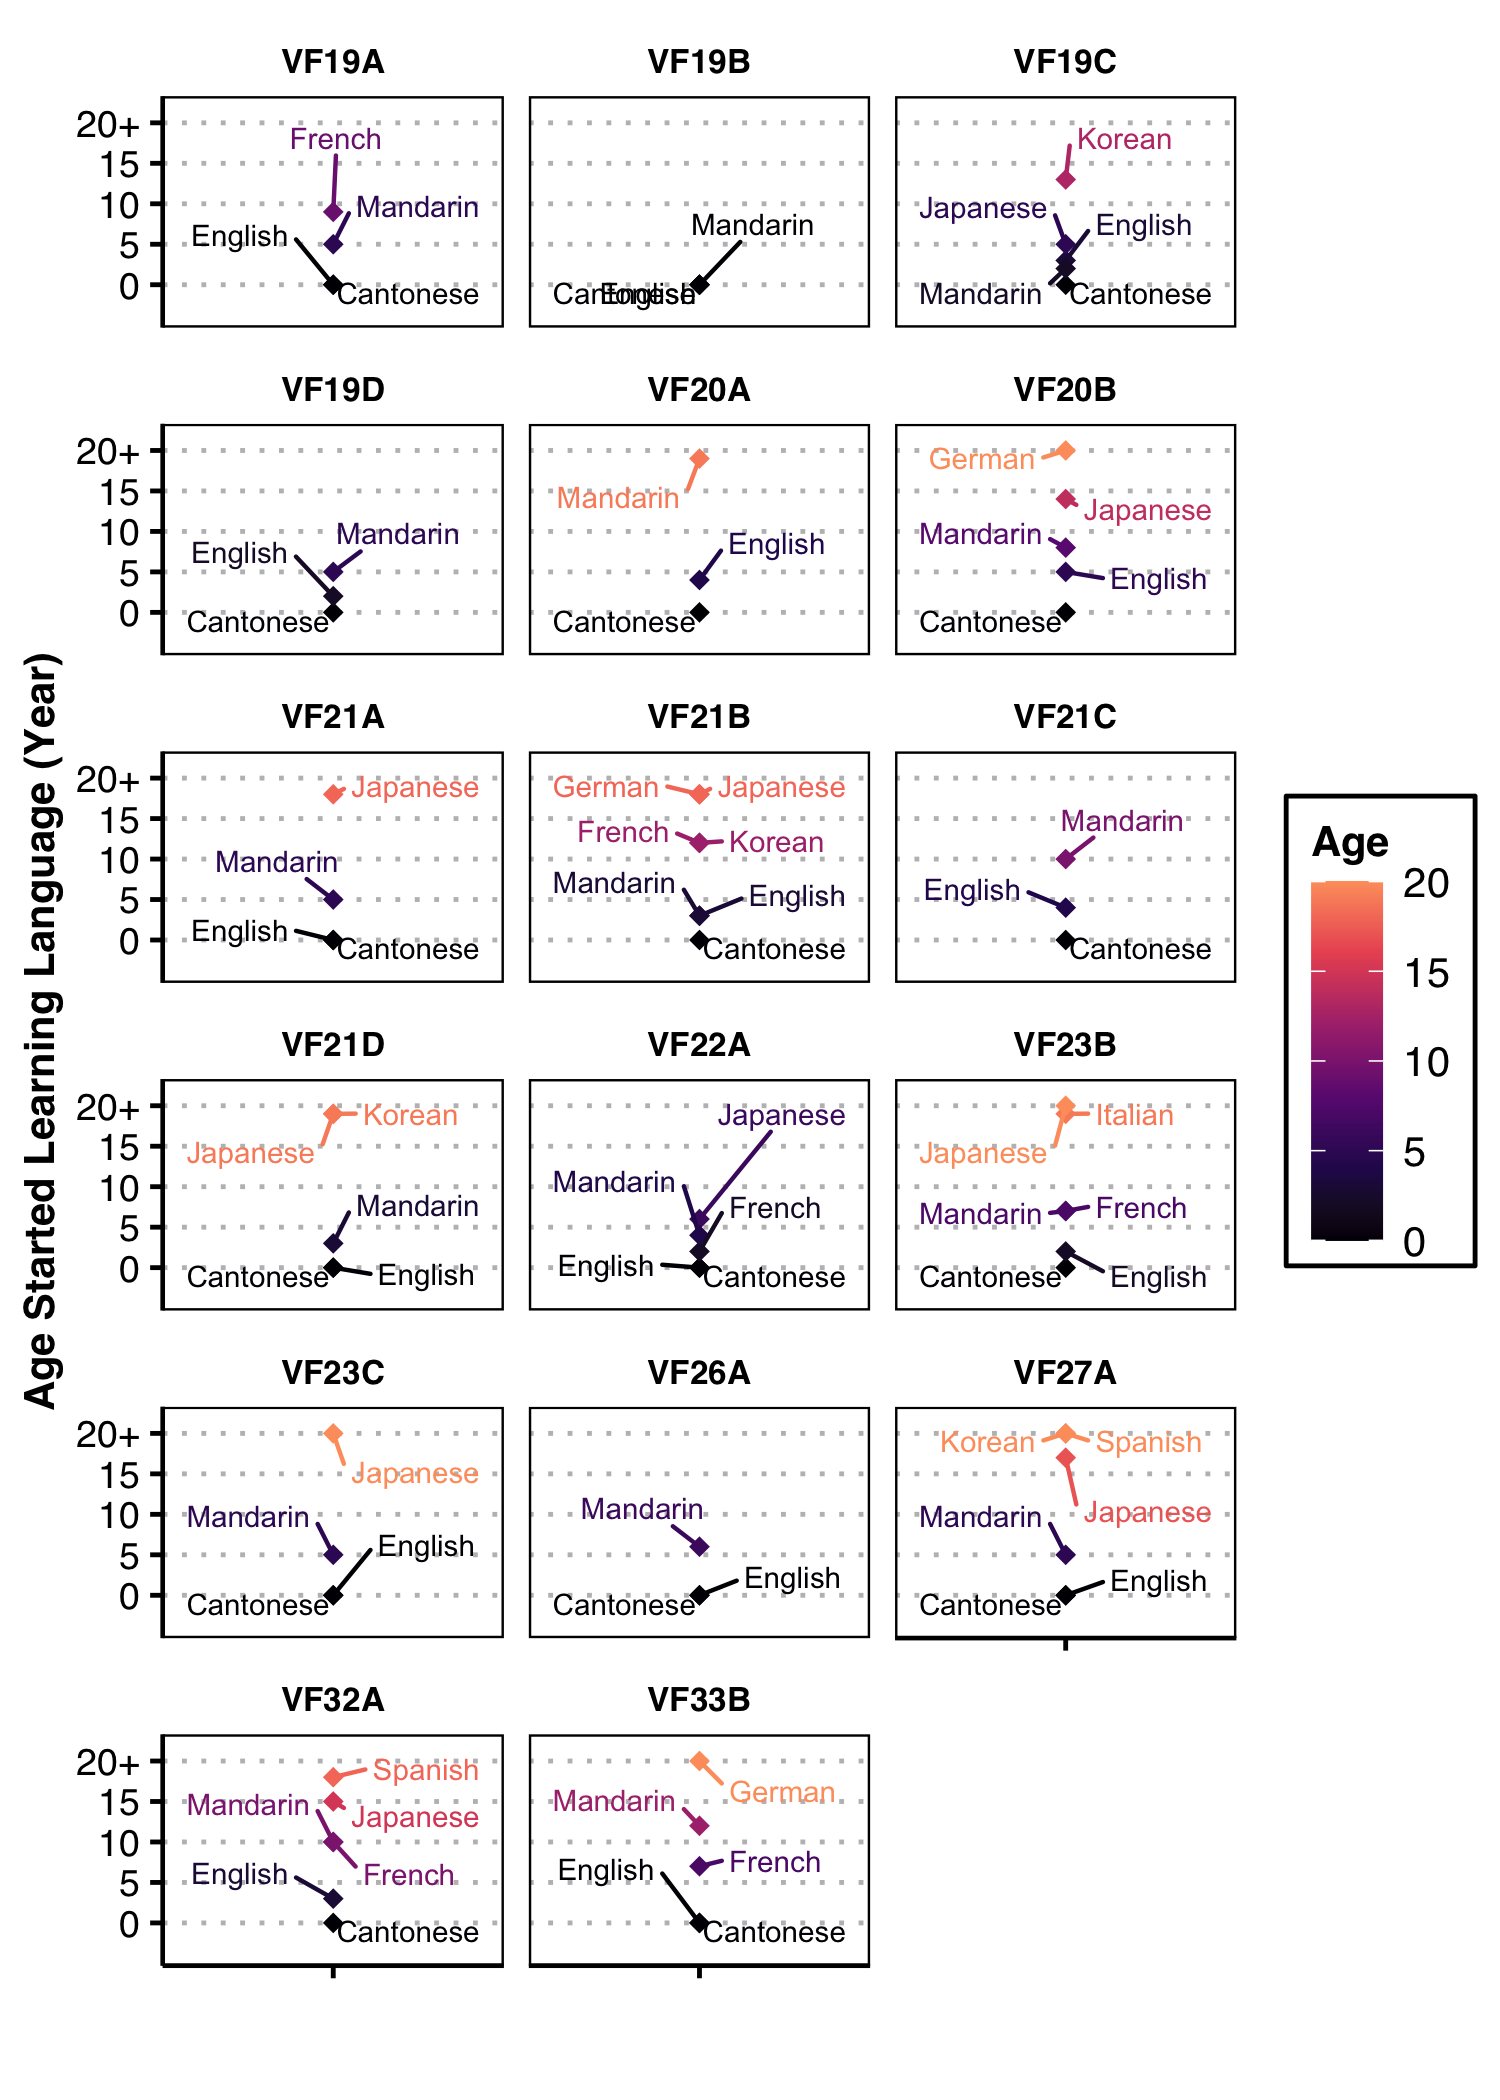
\includegraphics[width=4.5in]{figures/ch2_multilingualism_vf_5in.png} 
  \caption{Multilingualism for the female participants in the SpiCE corpus. Points represent the age that a participant began learning the language indicated in the label. Color is redundant with age, such that earlier ages are darker in color.}
  \label{ch2:fig:multilingualism_vf}
  \end{center}
\end{figure}

\begin{figure}[!htbp]
  \begin{center}
  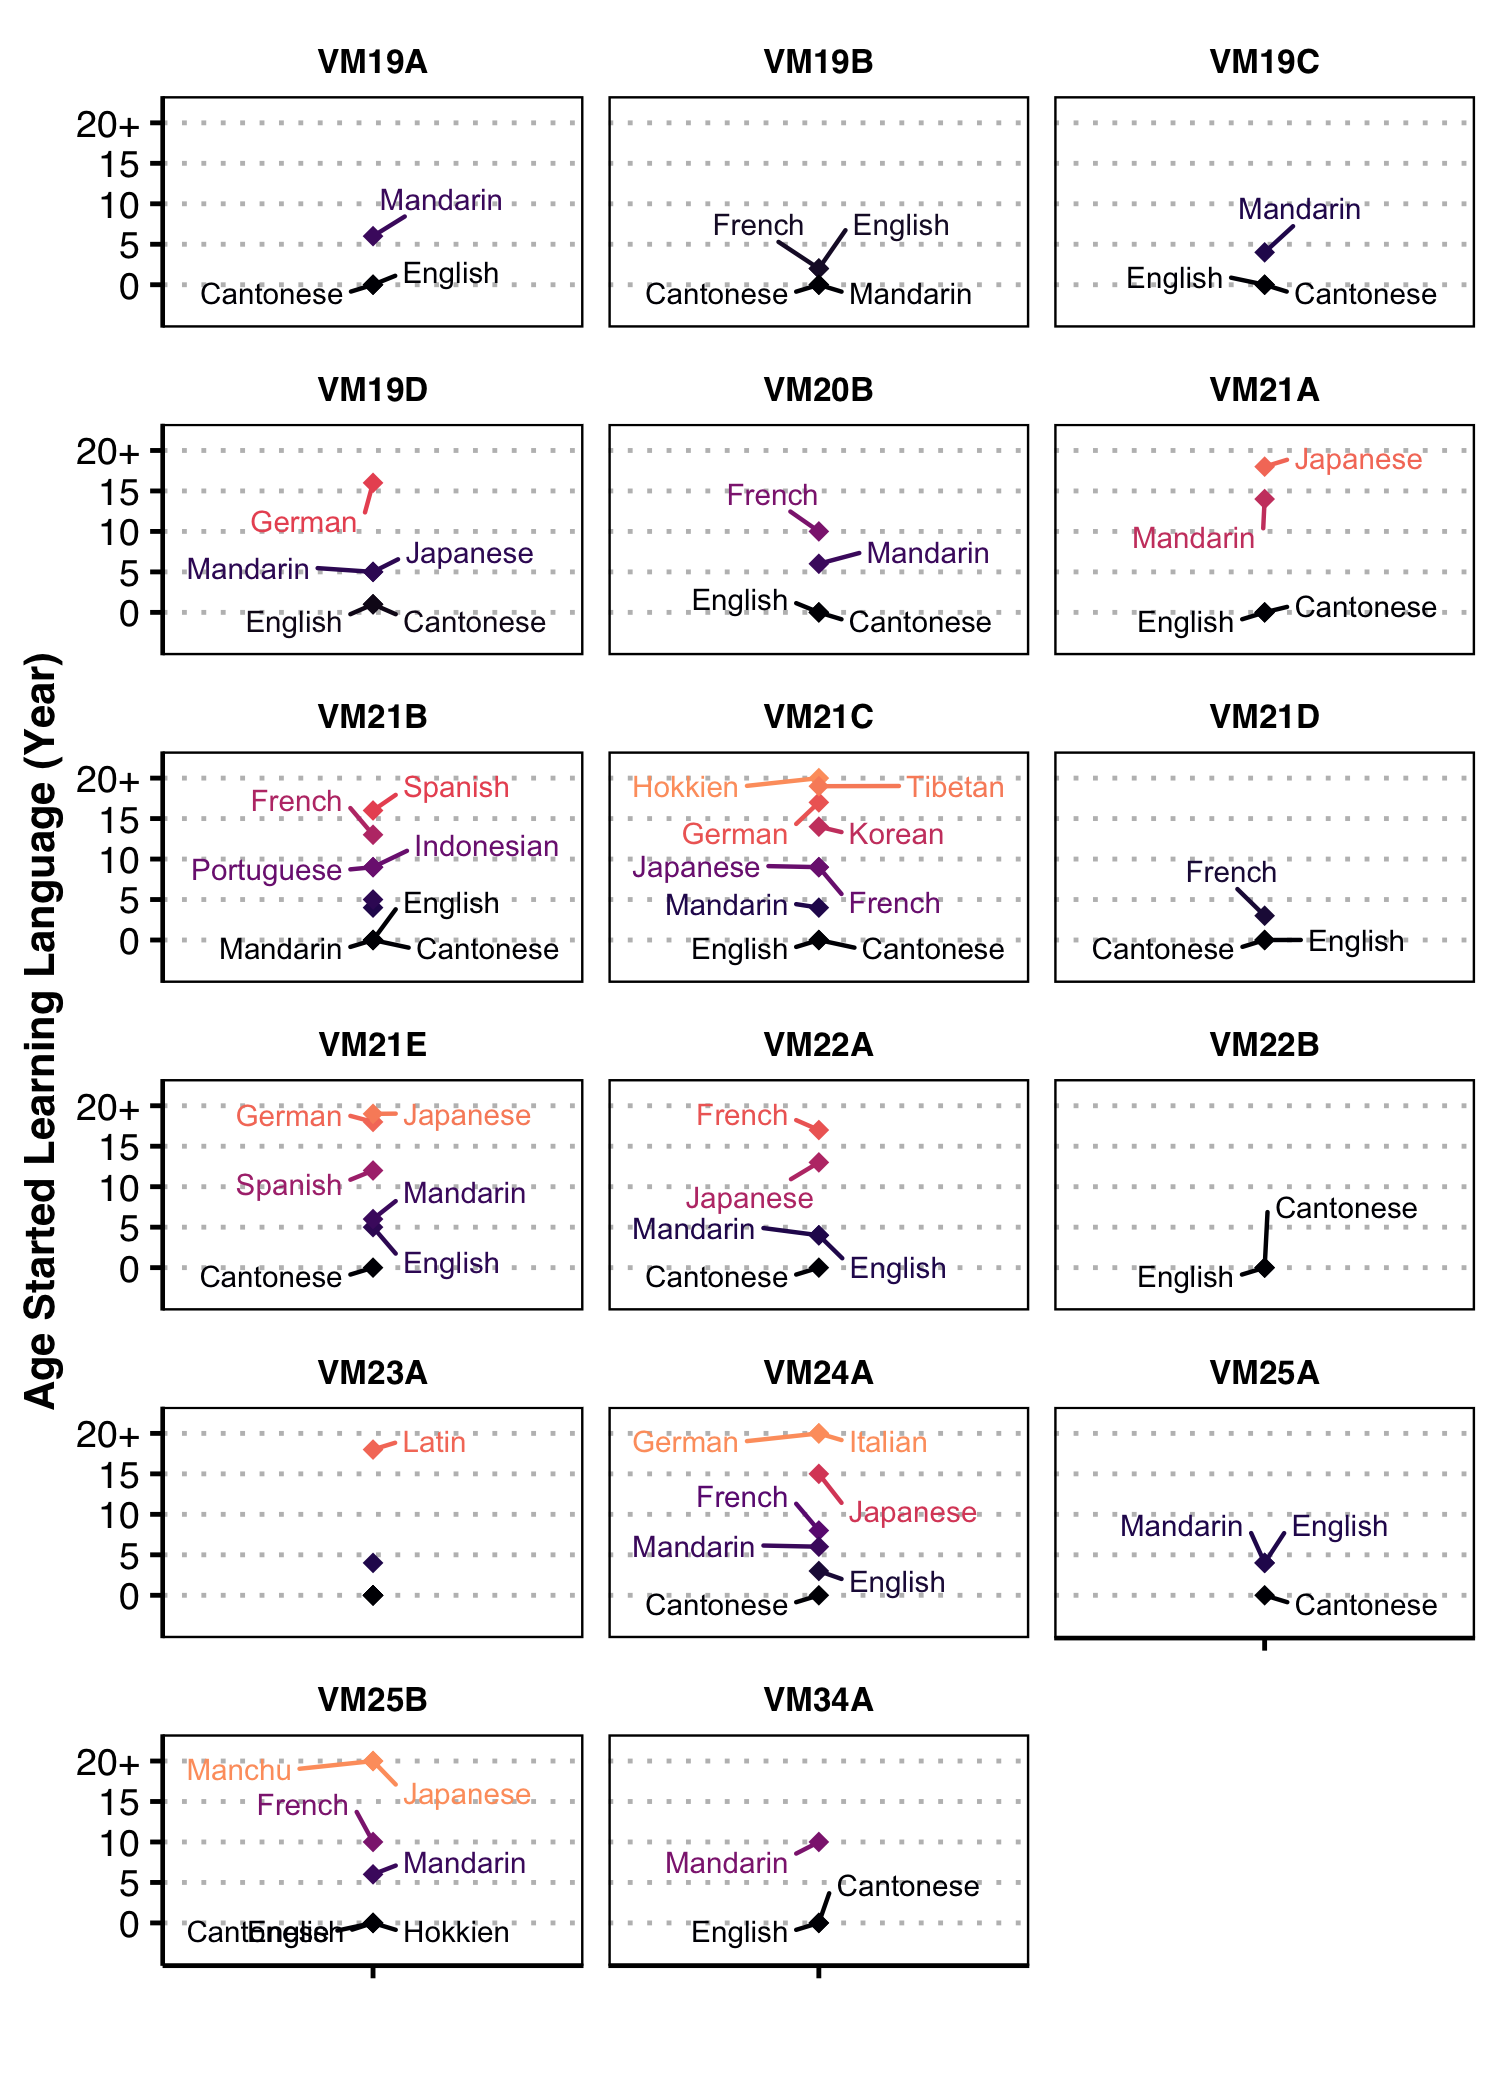
\includegraphics[width=4.5in]{figures/ch2_multilingualism_vm_5in.png} 
  \caption{Multilingualism for the male participants in the SpiCE corpus. Points represent the age that a participant began learning the language indicated in the label. Color is redundant with age, such that earlier ages are darker in color.}
  \label{ch2:fig:multilingualism_vm}
  \end{center}
\end{figure}

\subsection{Recording setup}\label{ch2:subsec:setup}

Recording took place in a quiet room in the linguistics laboratory building at the University of British Columbia in Vancouver, Canada. Two Cantonese-English undergraduate bilingual research assistants and the participant were seated around a table. The interviewer was a female Cantonese-English bilingual from Metro Vancouver. The recording process was monitored by a male Cantonese-English bilingual who grew up in Hong Kong and moved to Vancouver for university. The interviewer and participant were outfitted with AKG C520 head-mounted microphones positioned approximately 3 cm from the corner of the mouth. The microphones were connected to separate channels on a Sound Devices USBPre2 Portable Audio Interface. Stereo recordings were made with Audacity 2.2.2 \citep{audacity_2018_audio} on a PC laptop and saved with a 44.1 kHz sampling rate and 16-bit resolution.\footnote{Many files were originally recorded with 24-bit or 32-bit depth but were converted to 16-bit depth before the publication of the SpiCE corpus for the purpose of consistency and maintaining a reasonable file size while still providing high-quality audio.}

\subsection{Recording procedure}\label{ch2:subsec:procedure}

Upon arrival, participants were provided with an overview of the recording session procedures and informed of the corpus publication process. This included informing participants that they would be able to withdraw their data up until the SpiCE corpus' public release and that they would receive notice at least 30 days before publication.\footnote{No participants withdrew their data. When participants were notified of the upcoming corpus release, they were also encouraged to let the research team know if there were any portions of the interview they would like silenced from the published version.} Subsequently, participants were asked to provide written consent. Upon consent, participants completed a set of tasks in English and the same set of tasks in Cantonese---all within the same session. The order of languages was counterbalanced across participants (see Table~\ref{ch2:tab:participants}). This counterbalancing did not extend to other participant characteristics, and as a result, a higher proportion of the female participants completed the Cantonese part of the session before the English part and vice versa for the male participants. 
 
Each half of the session consisted of three tasks\textemdash sentence reading, storyboard narration, and a conversational interview\textemdash described in the following sections. While the primary focus of the recording session was the interview in each language, the sentence reading and storyboard narration tasks serve a practical purpose and add to the overall utility of the corpus. The rationale for each is described in the following sections. Each of these three tasks was recorded in the same audio file, though there are separate recordings for each half of the overall session. That is, each participant has a Cantonese recording and an English recording, each comprising the three tasks in that language. Together, each recording lasted approximately 30 minutes in each language. Along with the consent process, recording setup, and a break between interviews, participants spent up to 90 minutes in the lab. 

\subsubsection{Sentence reading}\label{ch2:subsec:sentences}
Sentence reading was included in the session to ensure that different participants produced a set of identical items, considering the core of the session was an unscripted, conversational interview (described in Section~\ref{ch2:subsec:interview}). While these sentences do not exhaustively reflect the sound systems of Cantonese and English, they provide samples of identical items for all individuals, which is advantageous for future analyses or projects that require matched utterances.

Participants first read the sentences listed in Table~\ref{ch2:tab:can_sent} and Table~\ref{ch2:tab:eng_sent} aloud, pausing between sentences. Participants completed a single repetition and were not instructed to speak in a particular style. As participants had varying levels of Cantonese reading ability, they were simultaneously presented with the Cantonese characters, Jyutping romanization, and English translation.\footnote{Jyutping is one of the primary Cantonese romanization systems \citep{matthews_2013_cantonese} and is widely used in Cantonese corpus research \citep{nagy_2011_hlvc, tse_2019_heritage}.} The Cantonese sentences were well-known declarative phrases, typically associated with Chinese New Year.\footnote{It is possible that familiarity and high frequency of some of these phrases led to them being produced with reduction patterns not present in a typical reading style---this is a limitation of the sentences.} While a more explicitly balanced set of sentences could have been used, participants' familiarity was deemed more important, as many Cantonese-English bilinguals in Canada are not literate in Cantonese. The English sentences included the Harvard Sentences list number 60 \citep{ieee_1969_sentences}, as well as a series of holiday-themed declarative sentences to better match the content of the Cantonese sentences. This task was relatively formal and typically lasted less than one minute in each language. 

In practice, the utility of these sentences may be somewhat limited, as sentences with speech errors were not necessarily repeated, and some Cantonese sentences were skipped altogether. In any case, the sentence reading task also served the purpose of getting participants into the appropriate Cantonese or English language mode before the upcoming interview. As such, they can be considered a warmup task. 

\begin{table}[!htbp]
\begin{center}
  \footnotesize
\begin{tabular}{c c}
\toprule
\textbf{No.}  & \textbf{English} \\
 \midrule
1 & Stop whistling and watch the boys march \\ 
2 & Jerk the cord, and out tumbles the gold \\ 
3 & Slide the tray across the glass top \\ 
4 & The cloud moved in a stately way and was gone \\ 
5 & Light maple makes for a swell room \\ 
6 & Set the piece here and say nothing \\ 
7 & Dull stories make her laugh \\ 
8 & A stiff cord will do to fasten your shoe \\ 
9 & Get the trust fund to the bank early \\ 
10 & Choose between the high road and the low \\ 
11 & Wish on every candle for your birthday \\ 
12 & Deck the halls with boughs of holly \\ 
13 & Ring in the new year with a kiss \\ 
14 & Have a spooky Halloween \\ 
15 & Enjoy the vacation with your loved ones \\ 
16 & Be filled with joy and peace during this time \\ 
17 & Relax on your holiday break \\ 
\bottomrule

\end{tabular}
\caption{Sentences 1\textendash10 comprise the Harvard Sentences List 60. Sentences 11\textendash17 are holiday-themed imperatives created for this corpus to match the Cantonese sentences thematically.}
\label{ch2:tab:eng_sent}
\end{center}
\end{table}

\begin{table}[!htbp]
\begin{center}
  \tiny
\begin{tabular}{cccc} %\begin{CJK}{UTF8}{bsmi}
\toprule
\textbf{No.} & \textbf{Cantonese} & \textbf{Jyutping} & \textbf{English translation} \\ 
\midrule
1 & 新年快樂 & \textit{san1 lin4 faai3 lok6} & Happy New Year \\ 
2 & 恭喜發財 & \textit{gung1 hei2 faat3 choi4} & Congratulations on happiness and prosperity \\ 
3 & 身體健康 & \textit{san1 tai2 gin6 hong1} & May your health be well \\ 
4 & 快高長大 & \textit{faai3 gou1 zoeng2 dai6} & Grow quickly \\ 
5 & 龍馬精神 & \textit{lung4 ma5 zing1 san4} & Have the spirit of the horse and dragon \\ 
6 & 學業進步 &\textit{ hok6 yip6 zeon3 bou6} & Progress in your education \\ 
7 & 年年有餘 & \textit{lin4 lin4 yau5 yue4} & Excess in each year \\ 
8 & 出入平安 & \textit{cut1 yap6 ping4 on1} & Leave and enter in safety \\ 
9 & 心想事成 & \textit{sam1 soeng2 si6 sing4} & Accomplish that which is in your heart \\ 
10 & 生意興隆 & \textit{saang1 yi3 hing1 lung4} & Have a prosperous business \\ 
11 & 萬事如意 & \textit{maan6 si6 yu4 yi3} & A thousand things according to your will \\ 
12 & 天天向上 & \textit{tin1 tin1 hoeng3 soeng6} & Upwards and onwards every day \\ 
13 & 笑口常開 & \textit{siu3 hau2 soeng4 hoi1} & Laugh with an open mouth frequently \\ 
14 & 大吉大利 & \textit{daai6 gat1 daai6 lei6} & Much luck and much prosperity \\ 
15 & 五福臨門 & \textit{mm5 fuk1 lam4 mun4} & Five blessings for your household \\ 
16 & 招財進寶 & \textit{ziu1 coi4 zeon3 bou2} & Seek wealth welcome in the precious \\ 
17 & 盤滿砵滿 & \textit{pun4 mun5 but3 mun5} & Basins full of wealth \\ 
\bottomrule
\end{tabular}
\caption{All Cantonese sentences are widely-known imperatives associated with Chinese New Year.}
\label{ch2:tab:can_sent}
\end{center}
\end{table}

\subsubsection{Storyboard narration}\label{ch2:subsec:storyboard}

For the second task, participants narrated a short story from a cartoon storyboard originally developed for linguistic fieldwork \citep{littell_2010_thank}. The storyboard followed a simple plot about receiving gifts and writing thank-you notes to family members and friends---a topic that Cantonese-English bilinguals in the corpus were expected to be familiar with in both languages. A reproduction of the storyboard is available with the corpus download. This task was less formal than the sentence reading task and ensured that different participants produced some of the same words in a more spontaneous context. Participants varied in how they approached this task, with some treating it as a series of picture description tasks and others taking a more narrative approach. Despite this difference, this task may be useful for future analyses or projects that require utterances in a matched semantic space, as participants narrated the same cartoon in each language. This ensured that some of the same content was conveyed in each language (e.g., productions of \textit{mother} in both languages). The storyboard narration lasted 4\textendash5 minutes in each session and allowed participants time to continue getting used to the recording setup. As with the sentences, the storyboard narration also facilitated participants getting into the language mode of the session before the conversational interview. This is important because language mode is known to affect the degree of crosslinguistic influence in speech production \citep{simonet_2019_convergence}.

\subsubsection{Conversational interviews}\label{ch2:subsec:interview}

The conversational interviews formed the bulk of the recording time for each participant, lasting around 25 minutes. Participants were informed of the general interview structure ahead of time. The casual interview format was inspired by the Buckeye corpus of conversational speech \citep{pitt_2005_buckeye} and included everyday topics such as family, school, culture, hobbies, and food. These topics were selected to be relevant, interesting, and encourage storytelling but to not delve into the personal details typically elicited in a sociolinguistic interview \citep{nagy_2011_hlvc}. A major goal was for participants\textemdash who knew they were being recorded for linguistic inquiry\textemdash to feel at ease and freely discuss the questions. Questions were loosely laid out under general topic headings, with optional follow-up questions. While the English and Cantonese interviews had the same structure and general topic areas, the particular questions differed. While within each language, the possible sequence of questions was the same, each interview took its own course, guided by what the participant wanted to talk about. This means that that the total number of general topics covered ranged from three to six. The interview materials are included with the corpus download. As a result, the speech samples from each language are comparable, but the specific questions differ between interviews and across participants. 

Participants were informed explicitly that code-switching was acceptable. Additionally, participants were implicitly encouraged to code-switch between languages by the interviewer, who included code-switches in some of her questions and asked about topics that encouraged switches (e.g., Chinese foods in English; university course work in Cantonese). While code-switching was encouraged, it was not a primary focus for the session. As will become apparent later in this chapter, there was substantially more code-switching in the Cantonese part of the session.

\begin{figure*}[ht]
\begin{center}
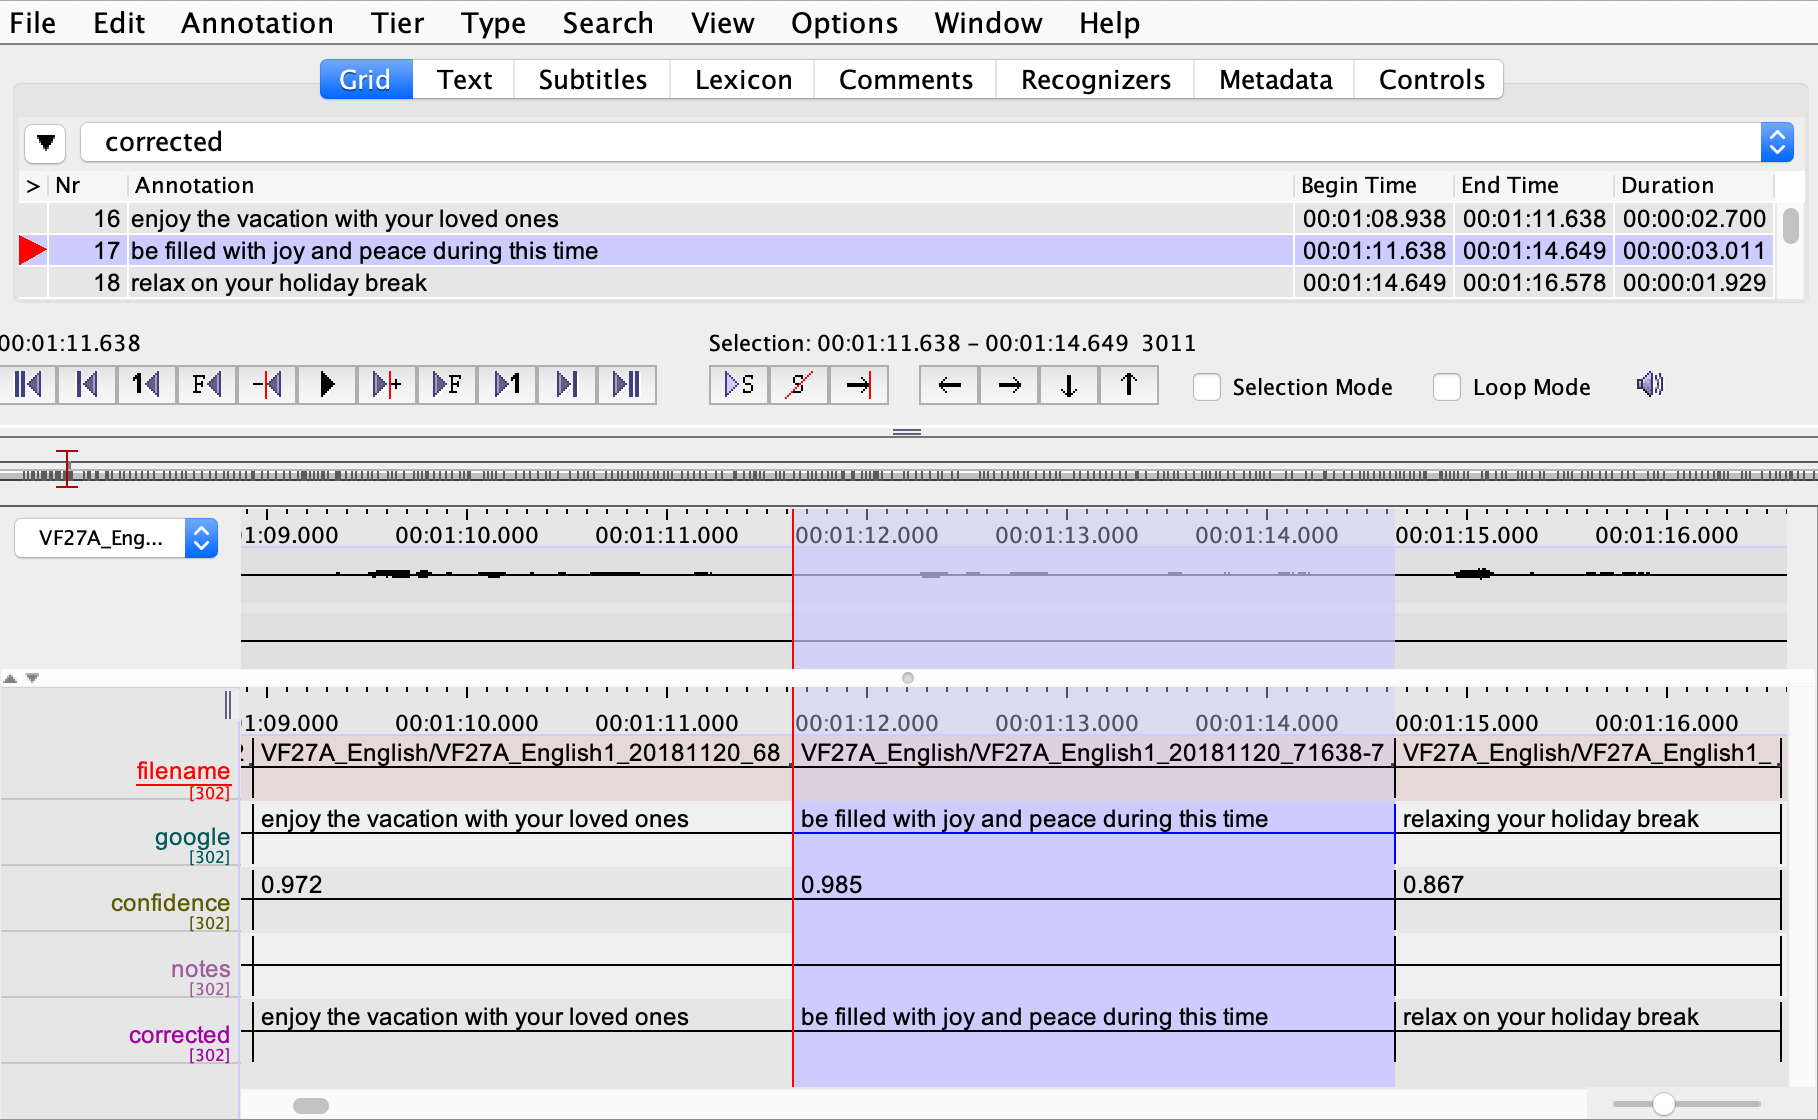
\includegraphics[width=4.9in]{figures/ch2_elan.png} 
\caption{This screenshot from ELAN shows a sample of hand-corrected English from the sentence reading task for participant VF27A. The audio waveform is displayed in two channels, with one for the participant (top) and the other for the interviewer (bottom). The annotation tiers include (1) the short audio chunk's filename, (2) the raw speech-to-text transcript, (3) the speech-to-text confidence rating, (4) space for transcriber notes, if any, and (5) the corrected transcript. Note that ``relaxing'' was corrected to ``relax on'' in the rightmost section displayed.}
\label{ch2:fig:elan}
\end{center}
\end{figure*}

\section{Annotation}\label{ch2:sec:annotation}
All recordings were processed according to the pipeline outlined in this section. As much as possible, automatic tools were leveraged to expedite manual correction. 

\subsection{Cloud speech-to-text}\label{ch2:subsec:stt}

Google Cloud Speech-to-Text was used to produce an initial transcript of the interviews \citep{google_2019_stt}. This was done using the Short Audio option, with the language variety set to Canadian English (en-CA) or Hong Kong Cantonese (yue-Hant-HK). To use this speech recognition product, the participant's speech was extracted from the participant's channel and segmented into short chunks, typically under 15 seconds in duration.\footnote{The interviewer's speech is included in the SpiCE corpus recordings for context but is not transcribed.} No attention was paid to constituents at this point; rather, breaks were placed at breaths and other pauses. Short chunks were necessary to use the speech recognition product with locally stored files, which was important for data privacy reasons. The short chunks would also prove useful for transcribers in the subsequent hand correction phase. With the audio files prepared in this way, speech recognition was completed using the Python client library for Google Cloud Speech-to-Text. The output included both a transcript and a confidence rating for each audio chunk. While the transcripts generated in this fashion were far from perfect, they served the function of expediting the hand-correction process.

\subsection{Orthographic transcription hand-correction}\label{ch2:subsec:orthographic}

The automatically generated transcripts were converted into multi-tiered ELAN transcription files \citep{sloetjes_2008_elan}, with tiers for the automatically generated transcript, phrase transcription confidence, notes, and corrected transcript. During hand correction, research assistants adjusted the transcript in the corrected tier and took note of anything pertinent to the given audio chunk. Figure~\ref{ch2:fig:elan} depicts an example of corrected English transcriptions in ELAN \citep{sloetjes_2008_elan}. Direct identifiers (e.g., names) were marked during this phase and silenced from the recordings prior to release. Transcriber guidelines were adapted from the multilingual Heritage Language Variation and Change corpus, which includes Cantonese \citep{nagy_2011_hlvc}. Guidelines for Cantonese were developed in collaboration with the bilingual research assistant team.

In both languages, the following conventions were used:
\begin{itemize}
 \item The placeholder ``xxx'' denotes unintelligible speech.
 \item Fragments are transcribed using ``\&'' followed by the fragment produced (e.g., ``\&s'').
 \item The ``?'' symbol marks questions but is not used consistently; other punctuation is not used.
\item Words produced in a language other than English or Cantonese are transcribed in the language with, for example, ``@m'' appended to the end of each form for Mandarin (simplified characters), ``@j'' for Japanese, ``@ml'' for Malaysian, and ``@i'' for Indonesian.

\end{itemize}

Cantonese-specific conventions include:
\begin{itemize}
 \item Where possible, transcription is in characters.
 \item Words without a standard character are transcribed in the Jyutping romanization system (e.g., \textit{jyut6ping3}).
 \item Fully lexicalized syllable fusion is transcribed with the smallest number of characters representing what was produced by the talker.\footnote{Syllable fusion is a phenomenon in which adjacent syllables in Cantonese are blended together. It ranges from assimilation at the syllable boundary to segment deletion and re-syllabification \citep{wong_2006_fusion}. Syllable fusion is common in Cantonese, though its frequency of occurrence and degree varies.} For example, when fully fused, 乜嘢 (\textit{mat1 ye5}, ``what'') is transcribed as 咩 (\textit{me1}). In some instances, an intermediate form is produced. For this lexical item, the intermediate form would be transcribed as 咩嘢 (\textit{me1 ye5}). Cases of fully lexicalized syllable fusion tend to be relatively clear to identify.
 \item Non-lexicalized (or ambiguous) cases of syllable fusion are transcribed with the full number of characters present in the un-fused form but with brackets identifying which syllables are fused. For example,  朝頭早 (``morning'') is pronounced \textit{ziu1 tau4 zou2} in its full form but can be fused to \textit{ziau14 zou2}---this fused form would be transcribed as 【朝頭】早. 
 \item Filled pauses are transcribed with the character 㖡 (\textit{e6}), or using Jyutping if different (e.g., \textit{m6}). 
 \item Transcribers followed a shared set of guidelines for transcribing sentence-final particles. This includes the following common particles:
    \begin{itemize}
      \item 呀 is the sentence-final particle used at the end of lists and for exclamations and questions.
      \item 呢 was used for both \textit{ne1} and \textit{le1} in marking questions.
      \item 囉 was used as a sentence-final particle for marking emphasis.
      \item 嚟 was the final particle used to expresses something being done or completed.
      \item 咗 was the particle used after verbs to mark past tense.
      \item While not a \textit{final} particle, 吖 was consistently used as a filler in the words 吖嗎 ``obviously'' and 吖嘛 ``isn't it.''
    \end{itemize}
\end{itemize}

English-specific conventions include:
\begin{itemize}
 \item Standard spelling is used.\footnote{While the goal was to use standard Canadian English spelling, given the range of transcriber backgrounds, the corpus includes some cases of American English spelling. This is relevant for a very small set of lexical items in the corpus (e.g., theater/theatre, favor/favour, etc.) }
 \item Proper nouns are capitalized (e.g., ``British Columbia''). 
 \item Filled pauses are transcribed with ``um'', ``er'', ``uh'', and other similar, non-elongated forms.
 \item Numbers are written out in word form (e.g., ``one hundred'').
\end{itemize}

\subsection{Forced alignment}\label{ch2:subsec:alignment}
Force-aligned transcripts were produced with the Montreal Forced Aligner \citep{mcauliffe_2017_mfa}, using the hand-corrected orthographic transcripts. The output of the forced alignment process was phone-level annotations for each audio file. Phones in this kind of transcript reflect a relatively broad level of transcription and are often referred to as phonemes in the context of acoustic models. While the definition of phoneme from each camp certainly has overlap between acoustic modeling and phonology, the two should not be equated.

In Cantonese, forced alignment was completed with the Train-and-Align option, as there was no pre-trained model available for Cantonese. As Cantonese orthography does not separate words with spaces, words segmentation was done using the \textit{jieba} Python library \citep{sun_2020_jieba}, along with a Cantonese word segmentation dictionary designed for use with \textit{jieba}.\footnote{The Cantonese Word Segmentation GitHub page: \url{https://github.com/wchan757/Cantonese_Word_Segmentation}.} While using an automated tool such as this is likely an imperfect solution, it has the benefit of reproducibility and consistency. This is important, as it can be difficult to define wordhood in Cantonese \citep[e.g., see][]{wong_2006_fusion}.

The Cantonese pronunciation dictionary was generated using the \textit{PyCantonese} Python library \citep{lee_2018_pycantonese}. Pronunciations were identified by getting the Jyutping romanization from each character or when transcription was done in Jyutping, using that existing Jyutping transcription. Next, the Jyutping was separated into segments, and the tone number was appended to the syllable nucleus (i.e., vowel or syllabic nasal). Research assistants supplemented the dictionary with alternative pronunciations for words that participated in syllable fusion. This approach bears some similarity to that of \citet{tse_2019_heritage} but differs in that it also includes tonal information---which has been shown to improve forced alignment as long as there are not too many tone-nucleus combinations \citep{cavar_2016_endangered, yuan_2014_automatic}.

Forced alignment in English took advantage of the Montreal Forced Aligner's pre-trained English model and pronunciation dictionary, which uses the ARPABET phone set. This dictionary broadly reflects North American English varieties. The dictionary was supplemented with manual additions to minimize the number of out-of-vocabulary items.

The word and phone output of the forced alignment process were included in a Praat TextGrid for each audio recording, along with annotation tiers for the task (sentences, storyboard, and interview) and utterance (the short chunks). In both sessions, any material not in the main language of the session was not force-aligned and appears as ``<unk>'' in the word tier and ``spn'' in the phone tier, representing unknown words and spoken noise respectively.\footnote{The Montreal Forced Aligner uses Kaldi conventions, and ``spn'' is short for ``spoken noise.'' While in some models, it can be used to represent specific kinds of spoken noise, it is used here as a catchall unknown phones.} The force-aligned transcripts were not manually corrected or checked. This means that any short chunk with code-switching or unintelligible speech will likely have poorer alignment because the model does not have a representation for that span of speech, either in the phone set or the pronunciation dictionary. As a result, it is advisable to use stringent exclusionary criteria or perform checks before analyzing data from the corpus. 

A sample output from one of the Cantonese interviews of the final corrected and force-aligned transcript is provided in Figure \ref{ch2:fig:praat}.

\begin{figure*}[htbp]
  \begin{center}
  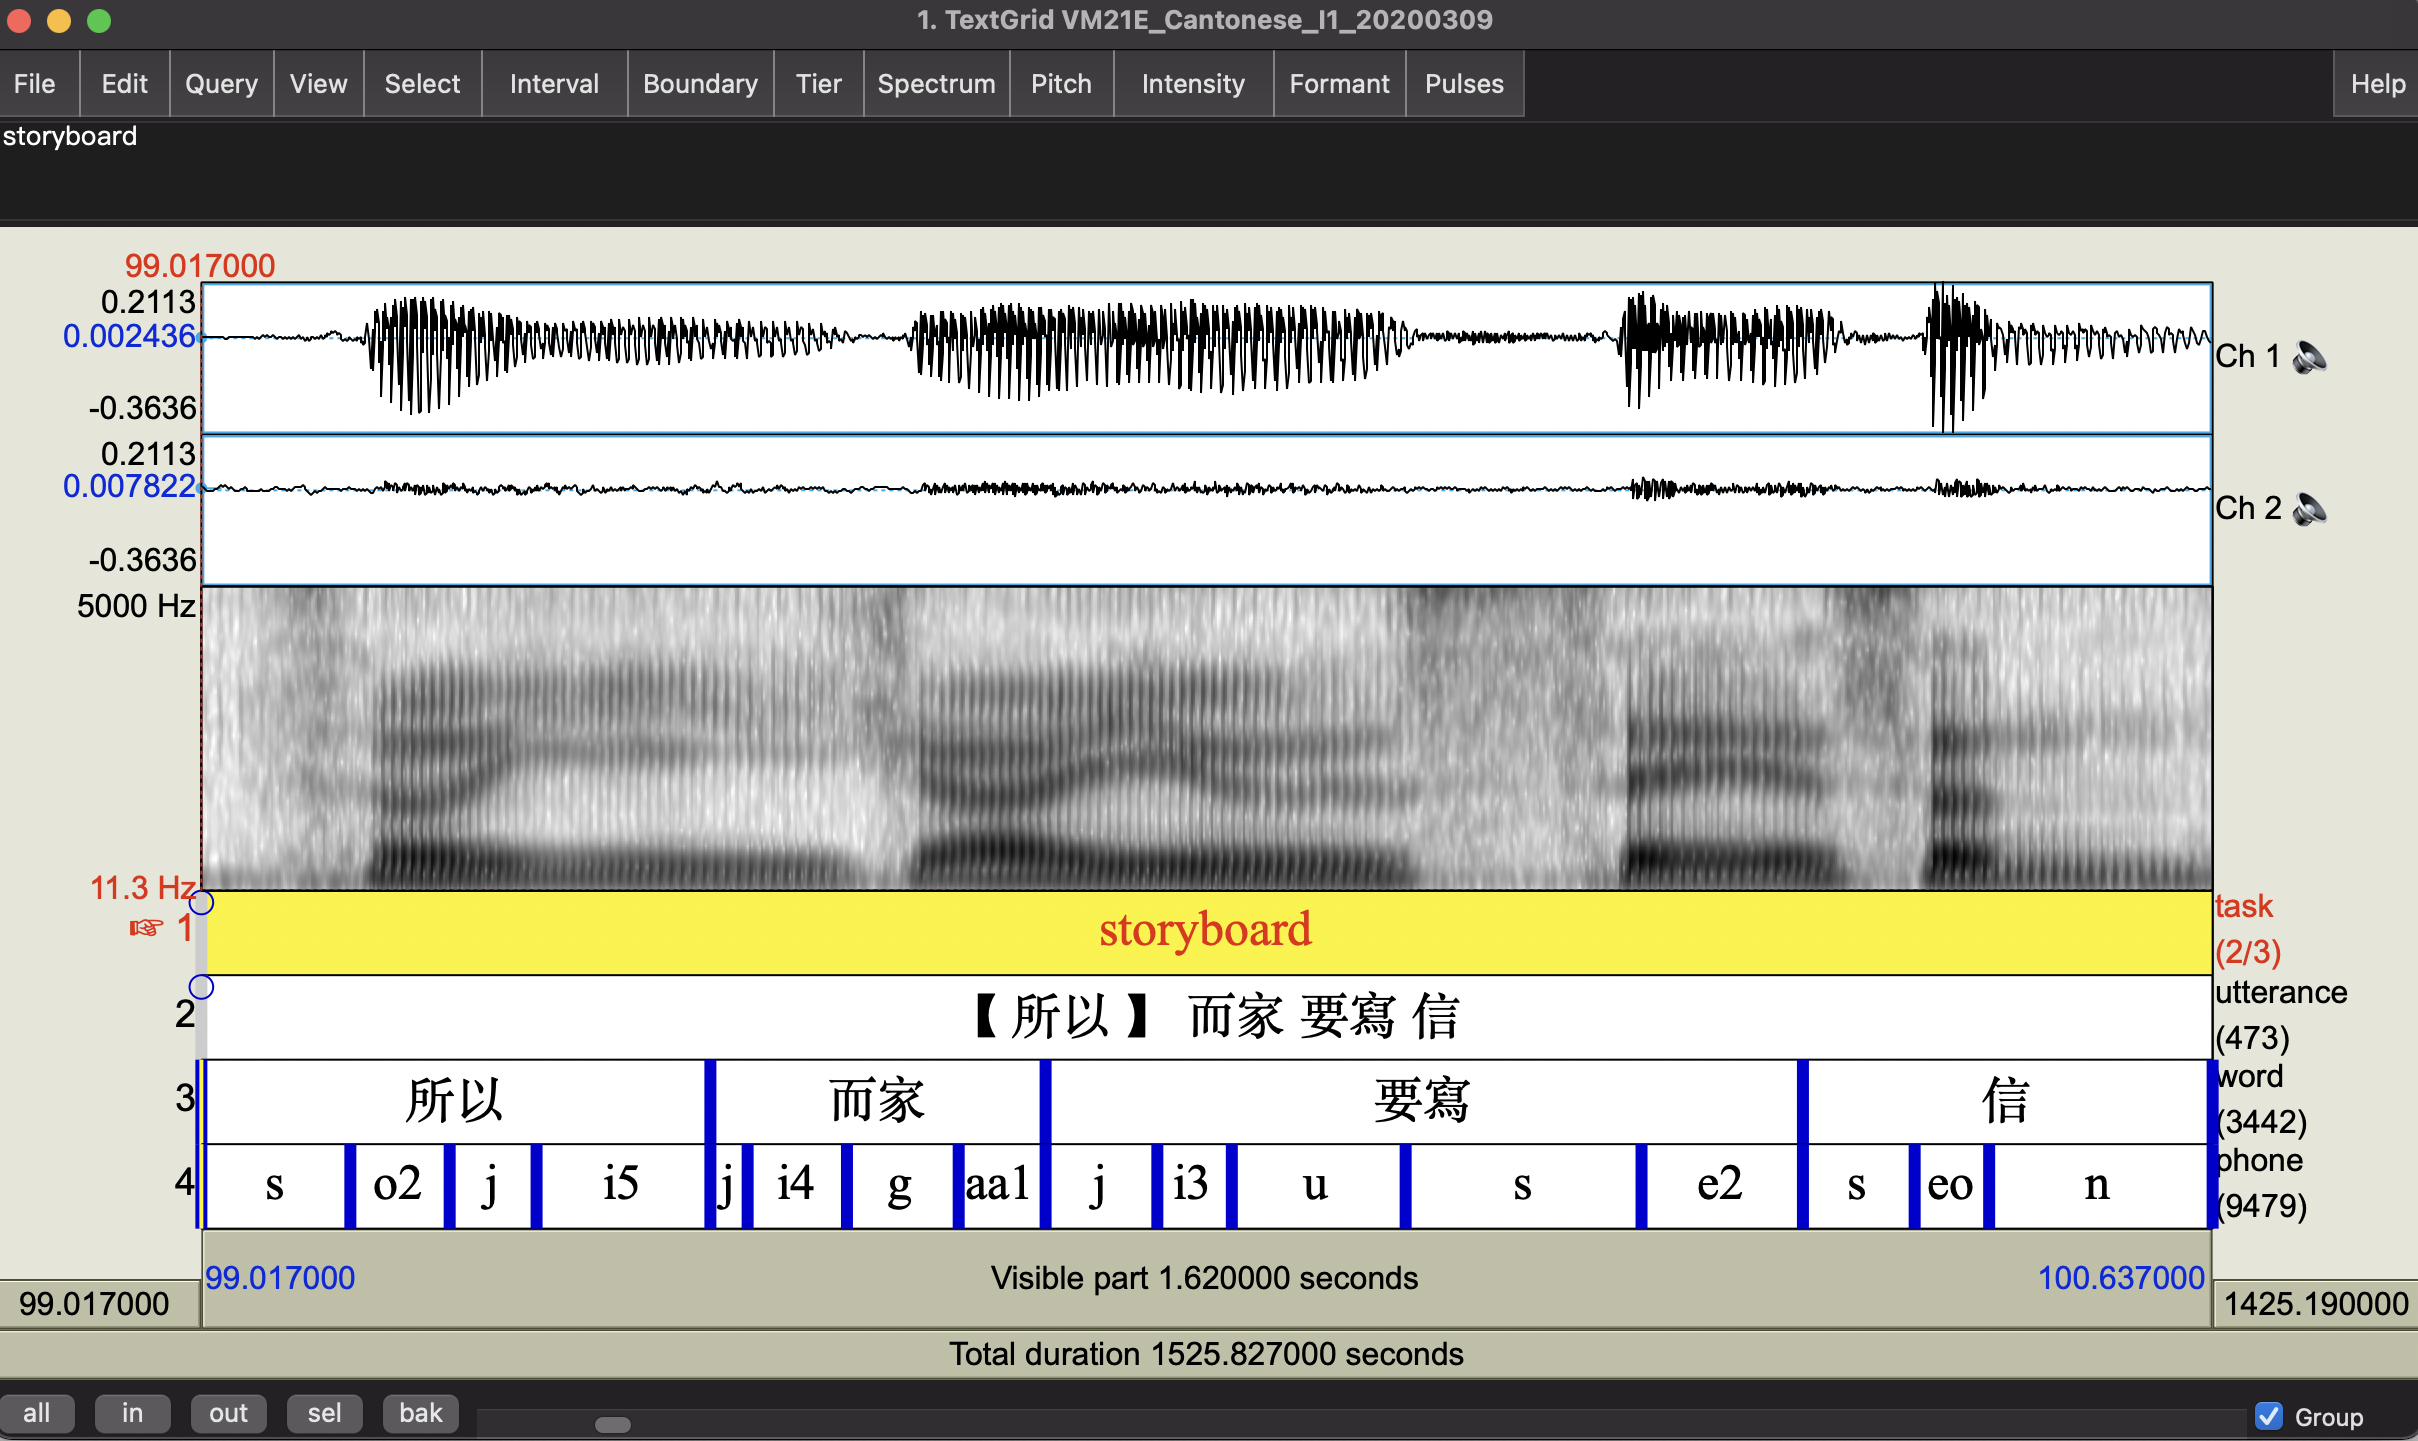
\includegraphics[width=\textwidth]{figures/ch2_praat_transcript.png} 
  \caption{This screenshot from Praat shows what the final transcript looks like for a small portion of a Cantonese interview.}
  \label{ch2:fig:praat}
  \end{center}
\end{figure*}


\section{Descriptive statistics}\label{ch2:sec:statistics}

The descriptive statistics in this section are intended to give a general sense of the quantity and quality of the data in the corpus. They are based on the transcript data as described in the previous section, specifically the hand-corrected utterance tier and the force-aligned phone tier. Additionally, this section only reports on participant speech, though the interviewer's speech is included in its own channel in the stereo audio files.

\subsection{Cantonese interviews}\label{ch2:subsec:cantonese_descriptive}

The Cantonese recordings include 8.3 hours of speech: 13.6 minutes of sentences, 44.0 minutes of storyboard narration, and 7.4 hours of conversational interview data. These estimates are calculated from the summed duration of all non-silent intervals in the phone tier of the transcripts, and as such, do not include interviewer questions or any pauses in the participant's speech. 

\begin{figure}[!htbp]
  \begin{center}
  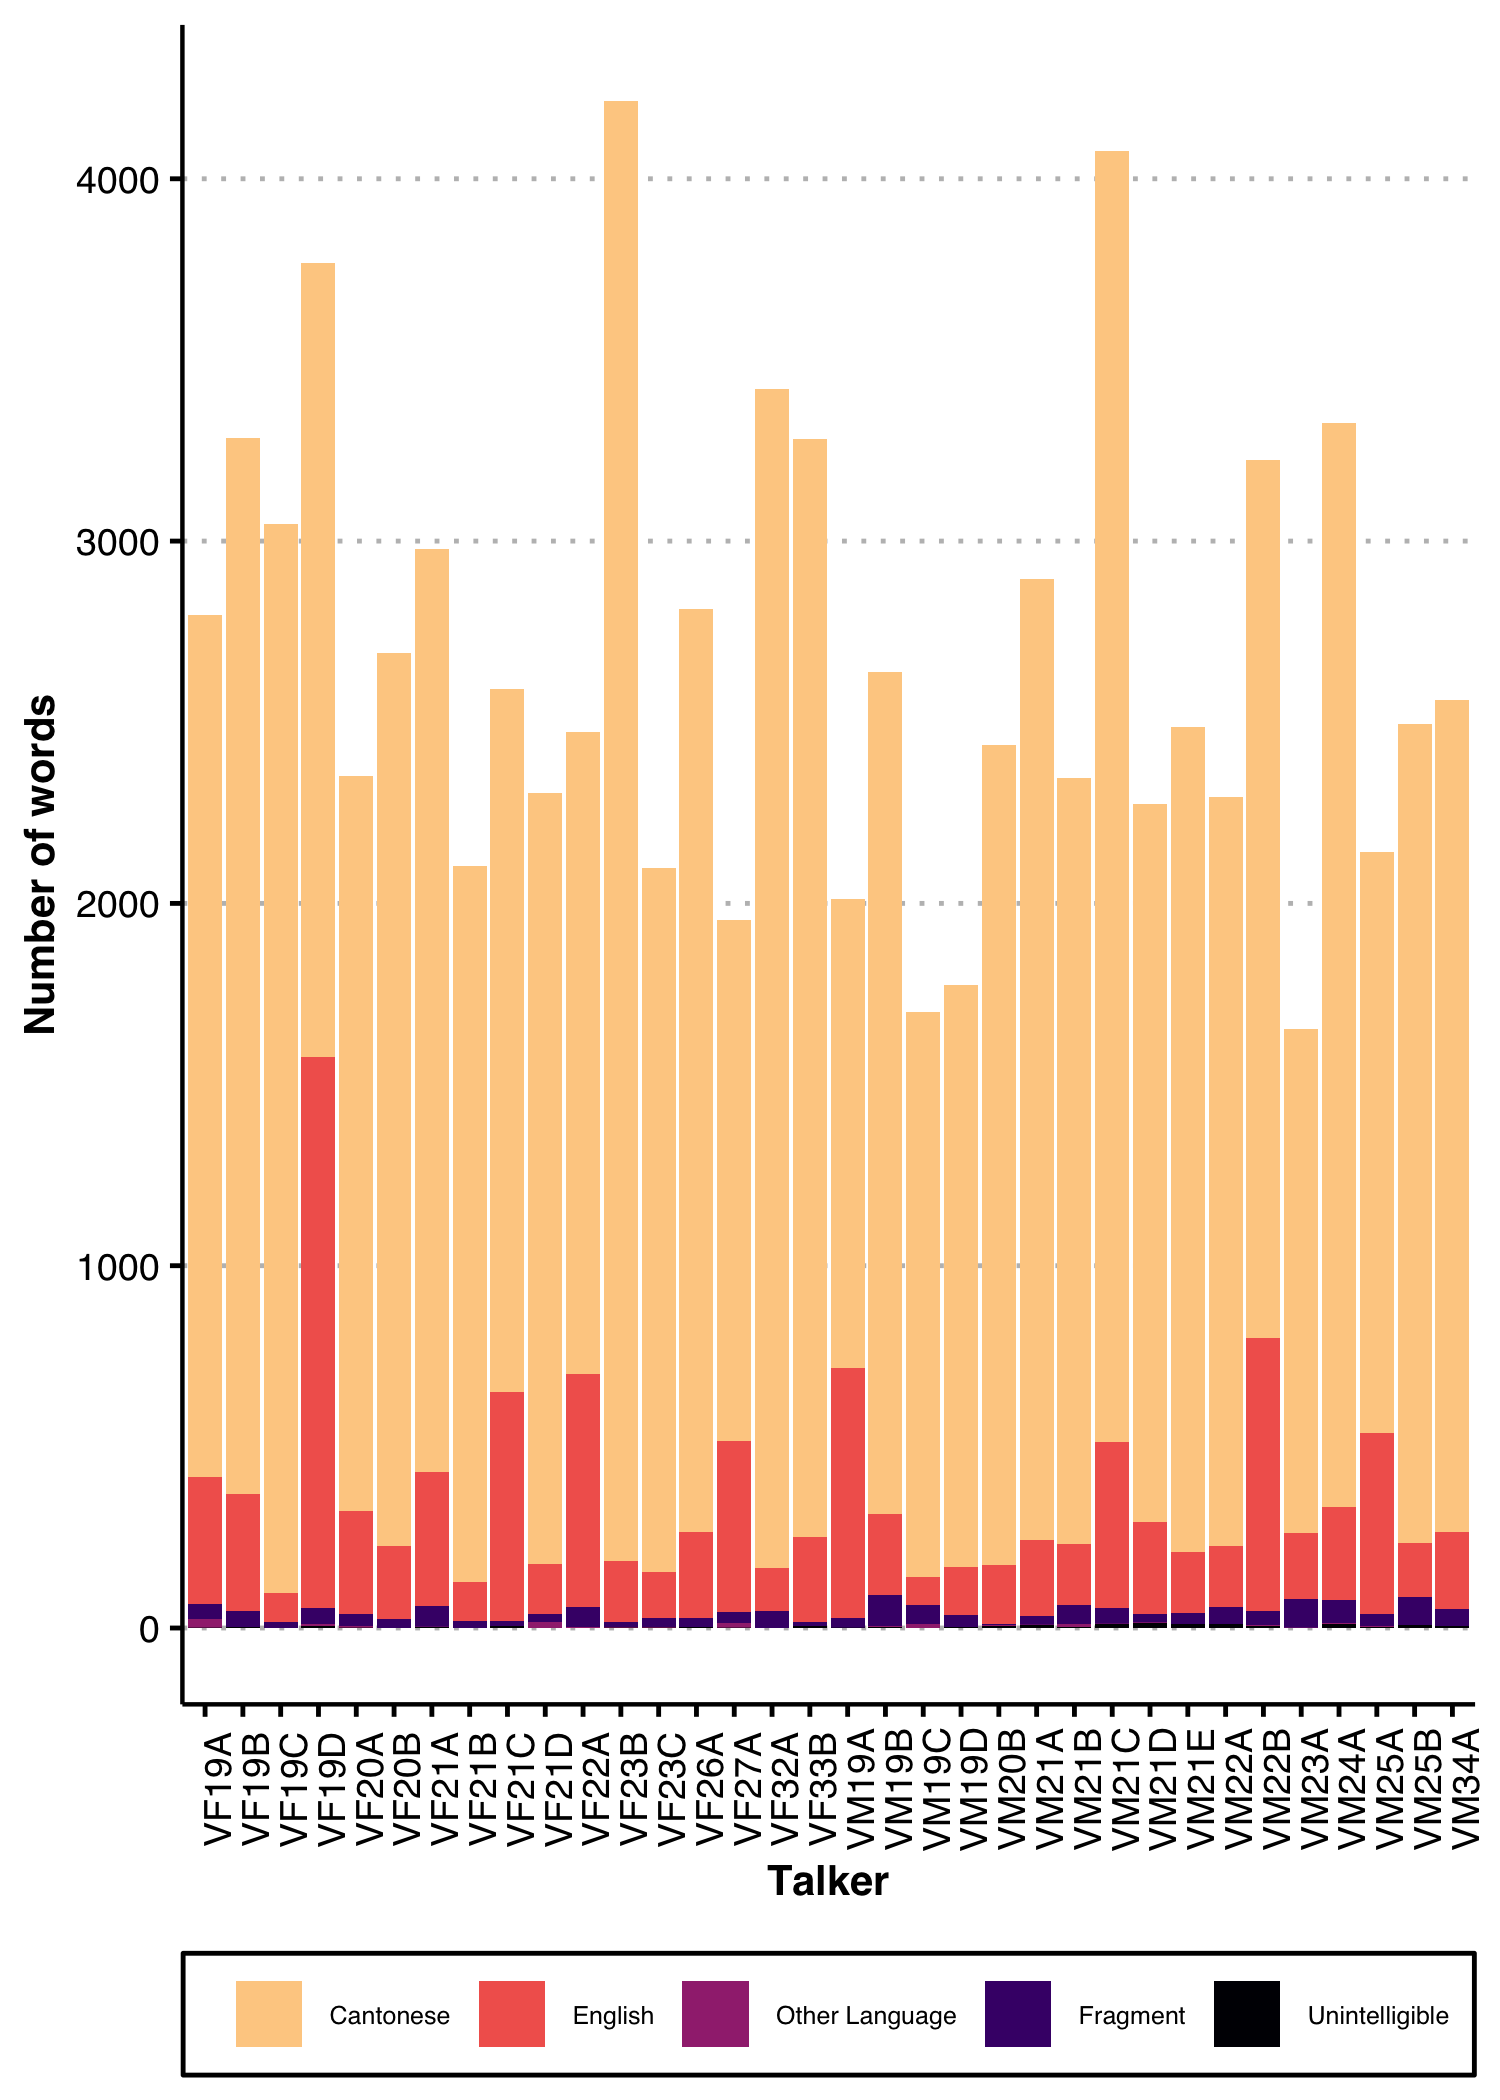
\includegraphics[width=4.9in]{figures/ch2_cantonesetypecounts_5in.png} 
  \caption{The total word count for each participant's Cantonese interview task is represented by bar height. Color indicates the kind of item counted. }
  \label{ch2:fig:cantonesetypecounts}
  \end{center}
\end{figure}

In the Cantonese interview sessions, there were a total of 8,112 word types and 90,512 word tokens. The number of words varies substantially across participants, with a mean of 749 word types (SD $=$ 157, minimum $=$ 483, maximum $=$ 1081) and 2,662 word tokens per interview (SD $=$ 6 37, minimum $=$ 1,654, maximum $=$ 4,212). The numbers reported here include all types of ``words''---Cantonese words, English words, words in other languages, phonological fragments, and unintelligible stretches of speech. Figure \ref{ch2:fig:cantonesetypecounts} shows the split of these categories on a by-participant basis within the Cantonese interview sessions. Figure \ref{ch2:fig:cantonesetypecounts} indicates that all participants switch to English during the Cantonese interview sessions. The amount of switching varies across participants, with VF19D producing an especially large number of English words. While the other three categories also vary, they are comparatively small in number. 

The overall distribution of word frequency in the Cantonese interviews is depicted in Figure~\ref{ch2:fig:cantonesewordfrequency}. As expected, there are a relatively small number of words occurring frequently (e.g., pronouns, function words, etc.), while a majority are mid- and low-frequency. This pattern follows what is expected in a word frequency distribution and is reassuring given the automated method of segmenting the Cantonese transcripts into words. 

\begin{figure}[ht]
  \begin{center}
  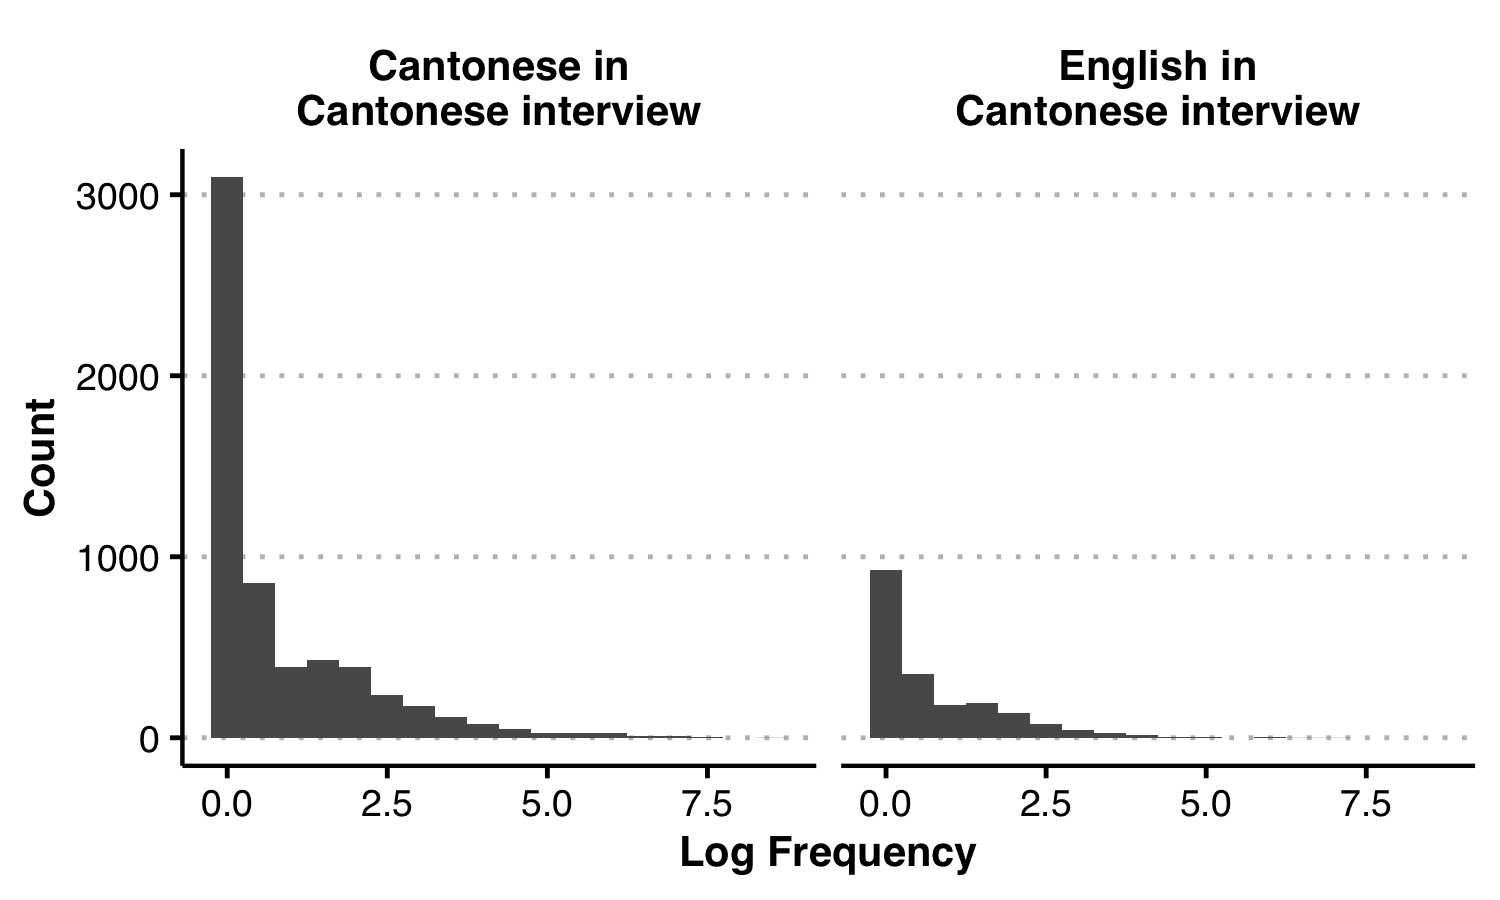
\includegraphics[width=4.9in]{figures/ch2_cantonesewordfrequency_5in.png} 
  \caption{The distribution of log word frequency for English and Cantonese words in the Cantonese interviews.}
  \label{ch2:fig:cantonesewordfrequency}
  \end{center}
  \end{figure}

\subsection{English interviews}\label{ch2:subsec:english_descriptive}

Using the same estimation technique as used for Cantonese, the English recordings include 8.9 hours of speech: 21.9 minutes of sentences, 45.7 minutes of storyboard narration, and 7.7 hours of conversational interview speech.

The English interviews include a total of 4,972 word types and 104,618 word tokens. As in the Cantonese interviews, the number of words varies substantially by participant, with a mean word type count of 609 (SD $=$ 119, minimum $=$ 434, maximum $=$ 904) and token count of 3,077 (SD $=$ 701, minimum $=$ 1,907, maximum $=$ 4,240). Figure \ref{ch2:fig:englishtypecounts} shows the split of these categories on a by-participant basis within the English interview sessions. Unlike the Cantonese interviews, there were relatively few switches to Cantonese, with 12 of the 34 participants producing fewer than 10 Cantonese words during the English sessions.

The distribution of log word frequency for both Cantonese and English words in the English interviews is portrayed in Figure~\ref{ch2:fig:englishwordfrequency}. Word frequency follows a similar pattern to Cantonese word frequency, with most words occurring infrequently and a smaller proportion occurring very frequently.

\begin{figure}[th]
  \begin{center}
  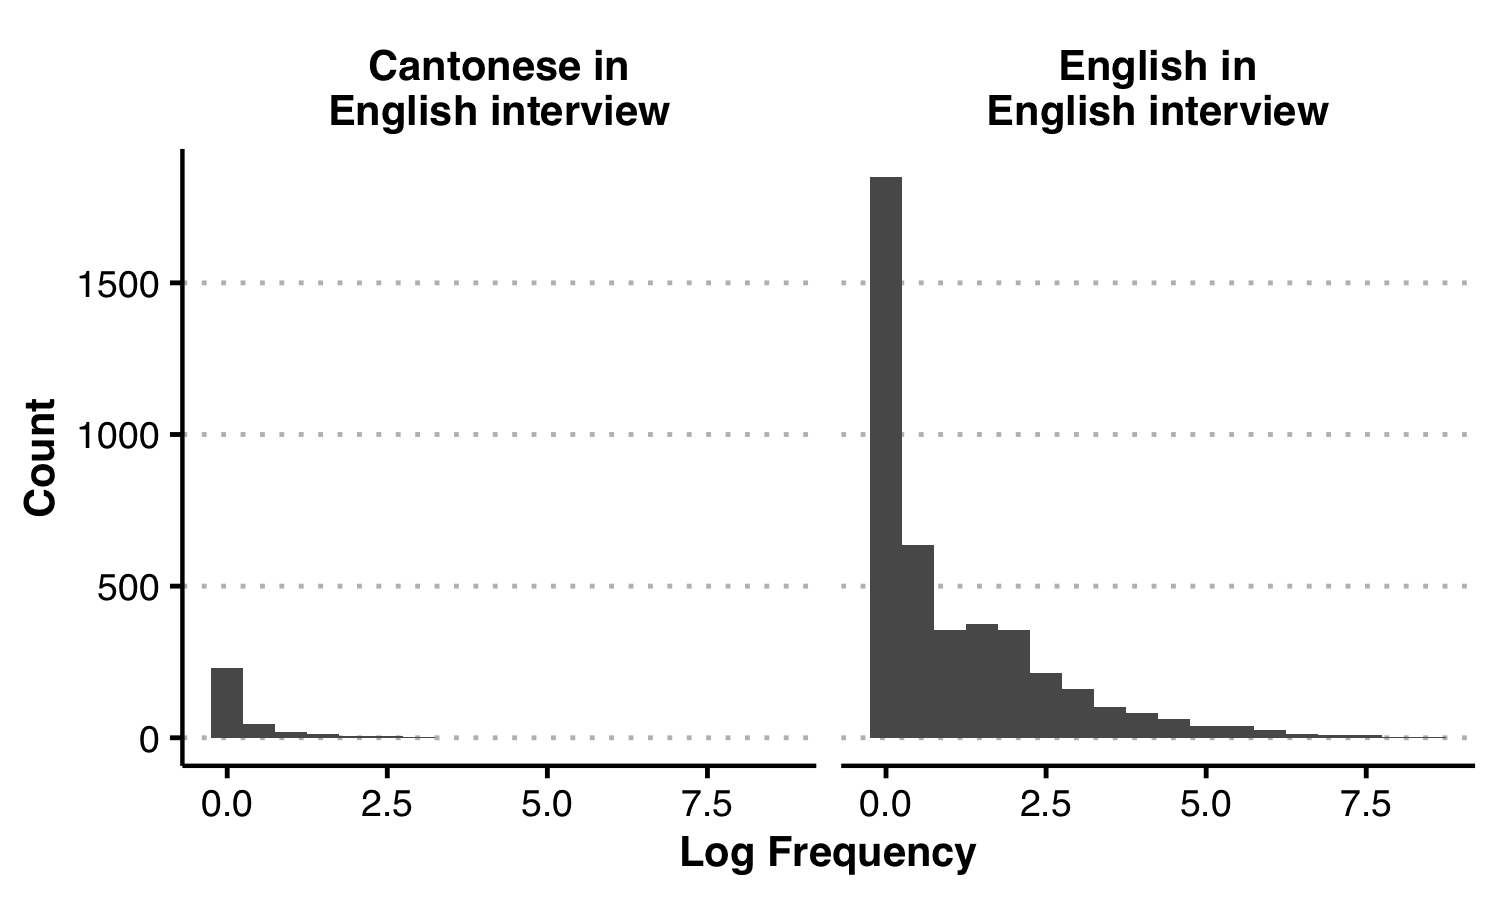
\includegraphics[width=4.9in]{figures/ch2_englishwordfrequency_5in.png} 
  \caption{The distribution of log word frequency for English and Cantonese words in the Cantonese interviews.}
  \label{ch2:fig:englishwordfrequency}
  \end{center}
\end{figure}

\begin{figure}[!htbp]
  \begin{center}
  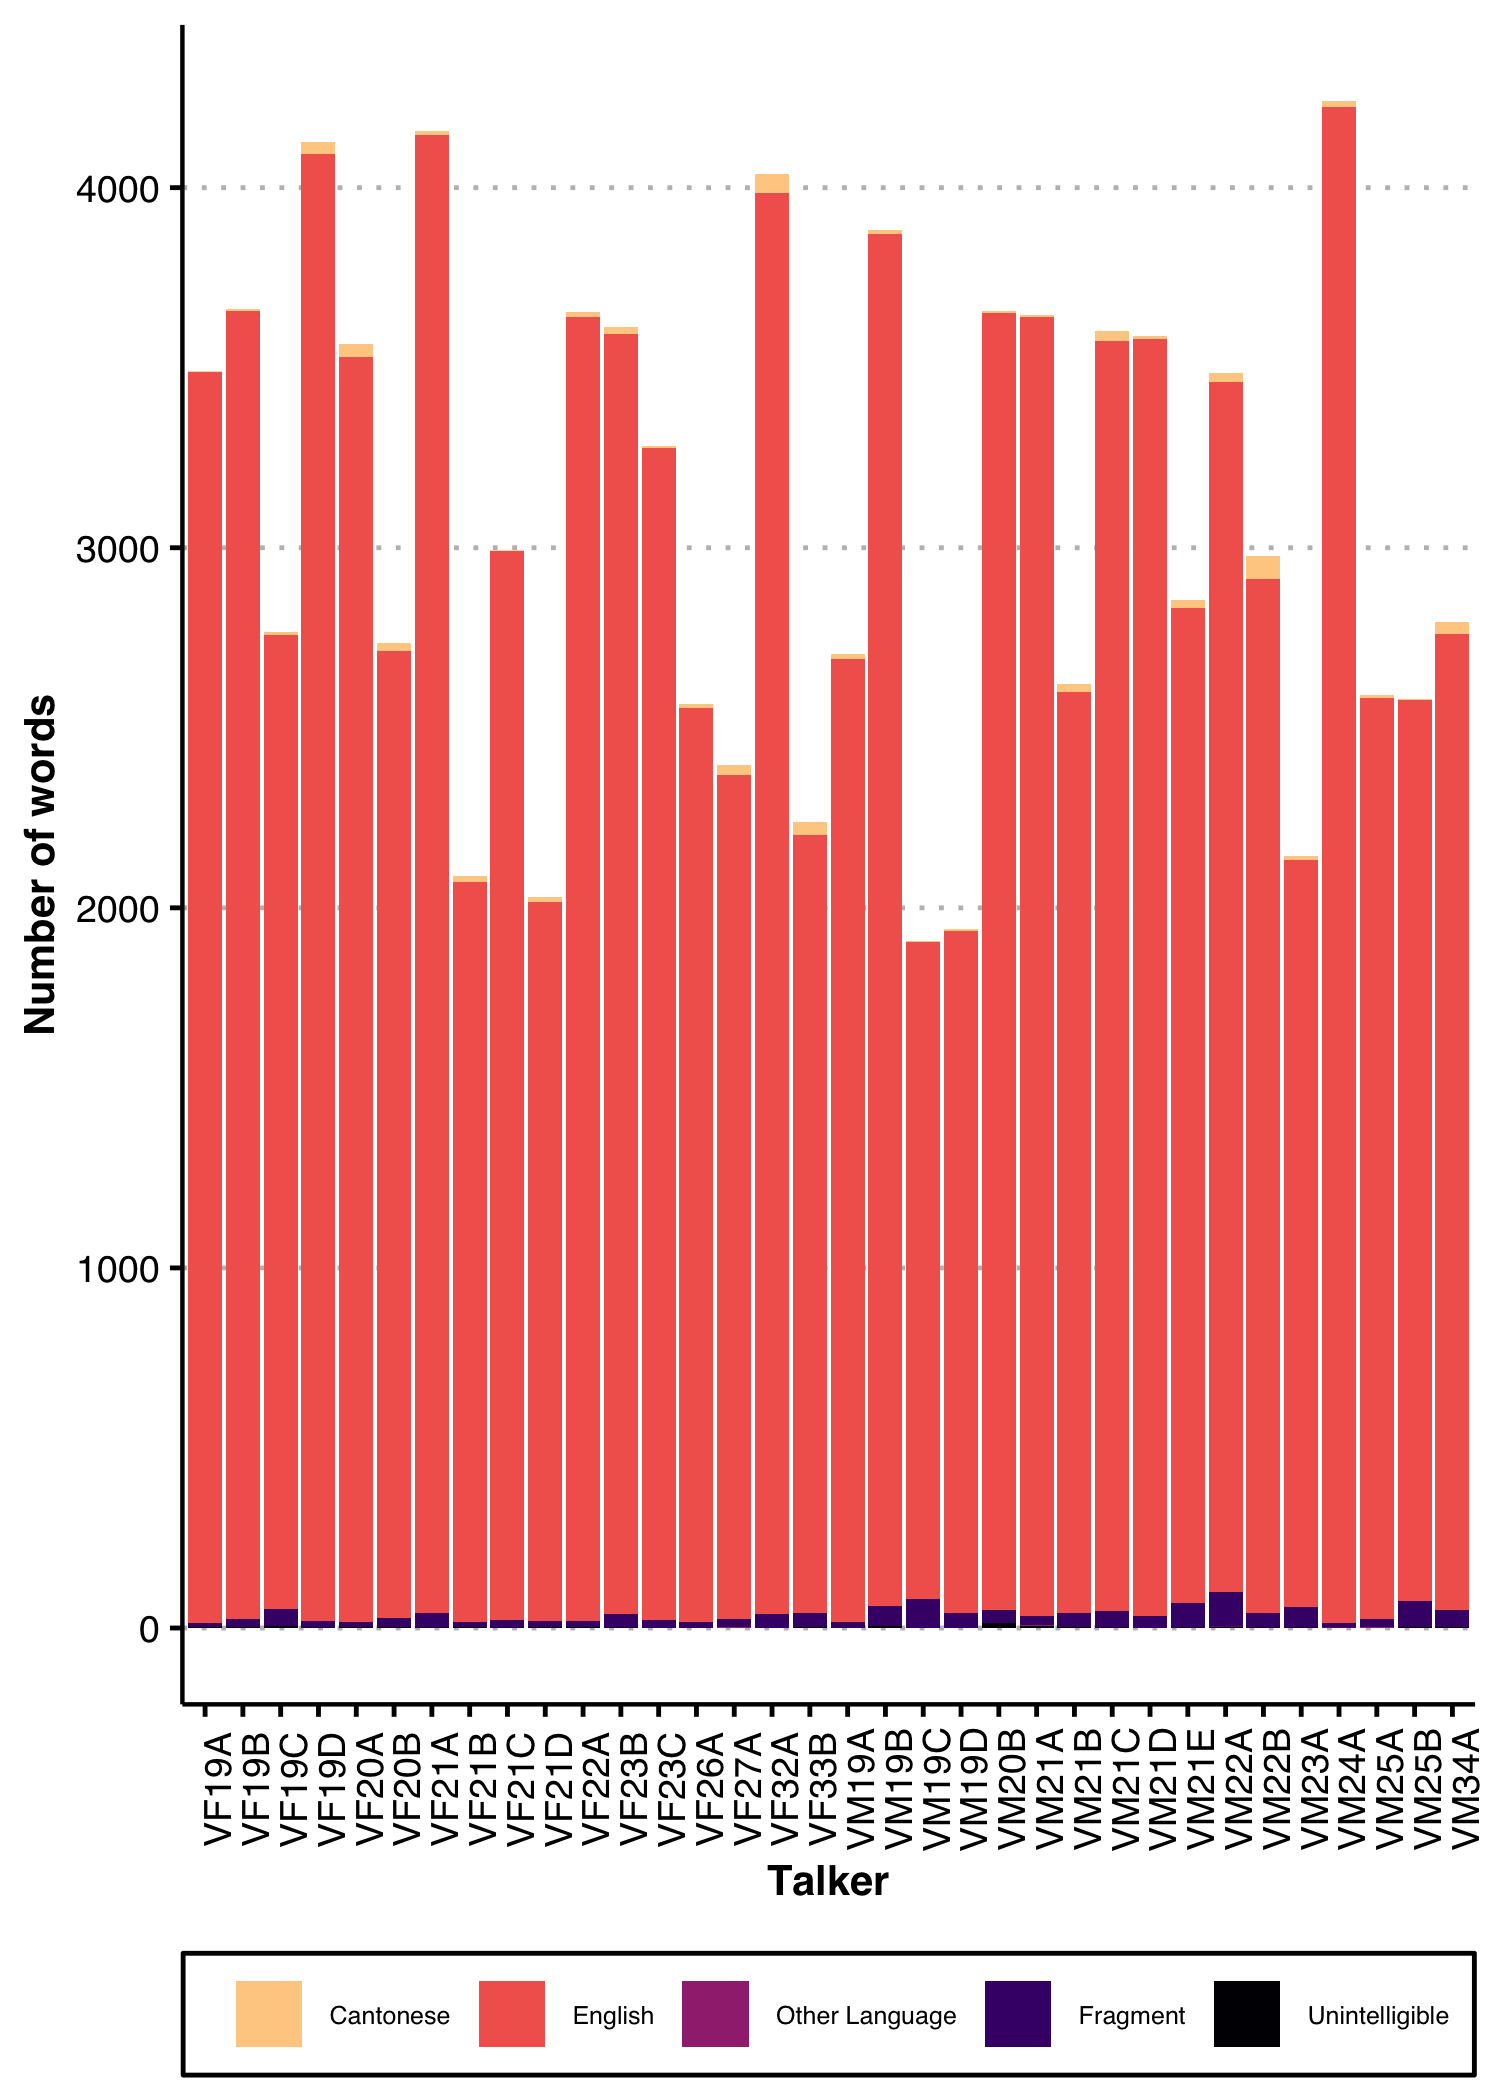
\includegraphics[width=4.9in]{figures/ch2_englishtypecounts_5in.png} 
  \caption{The total word count for each participant's English interview task is represented by bar height. Color indicates the kind of item counted. }
  \label{ch2:fig:englishtypecounts}
  \end{center}
\end{figure}

\section{SpiCE corpus release}\label{ch2:sec:releases}

The SpiCE corpus was publicly released in May 2021 through the Scholars Portal Dataverse platform under a Creative Commons Attribution 4.0 International License.\footnote{\url{https://creativecommons.org/licenses/by/4.0/}} In addition to the corpus itself, documentation is available online---the URLs are given in Section \ref{ch2:sec:design}.

\section{Discussion and conclusion}\label{ch2:subsec:discussion}

While various bilingual corpora exist, they lack in different ways \textit{for the purpose of doing corpus phonetics}. The SpiCE corpus described here enables within-speaker phonetic comparisons across languages. While this would be possible with some of the bilingual speakers in resources like the Bangor corpora \citep{deuchar_2014_corpora}, the recording quality in such resources limits the scope of phonetic research. With the release of SpiCE and its high-quality recordings, scholars can ask and answer empirically and theoretically motivated research questions within the speech and language sciences using more sophisticated phonetic measurement techniques (e.g., spectral measures, in addition to temporal measures). This presents substantial potential for increasing our understanding of bilingual spoken language from both phonetic and psycholinguistic perspectives. While the recording quality of this corpus offers these particular advantages, SpiCE is also suitable for any other standard corpus-based inquiry with conversational speech, whether linguistic or paralinguistic in nature. The opportunities made available with SpiCE are especially important given the typological difference between the languages under consideration and the fact that Cantonese is an understudied language. 

\endinput % -------------------------------------------------------- %
